\section{The four-change observable}
\label{sec:observable}

We determine the probability of the two connection alternatives in a
fixed polygon with four alternating boundary designations.  The finite
boundary-tree calculation produces a bounded observable and identifies
its possible boundary values.  Two analytic steps remain: remove a
diagonal correction from those values, and prove that every interior
limit is holomorphic.  Both steps use matched interior and exterior
walls, with positive normalizations that retain the growth of local
loop weights.  The resulting boundary problem has a strictly convex
target and determines the connection probability.

The analytic inputs are the disk and screening estimates of
Section~\ref{sec:disks}, the local tilt bounds of
Section~\ref{sec:angular}, and the physical current and charge estimates
of Section~\ref{sec:physical}.  The output here is the exact
compatible-mesh polygon formula in Theorem~\ref{thm:fixed-polygon}.
Section~\ref{sec:moving} will transfer it to varying and slit domains.

The four-boundary-change FK-Ising construction of Chelkak and Smirnov
\cite[Section~6]{ChelkakSmirnov2012} is an antecedent of this auxiliary
pairing problem.  We give the finite calculation and the below-one
analytic estimates needed for the present parameter range.

\subsection{The four-mark boundary tree}

Fix $0<q<1$, $d=\sqrt q=2\cos\lambda$, and
$\rho=\lambda/\pi\in(1/3,1/2)$.  Let $\Omega$ be a fixed rational
simple orthogonal polygon in tile coordinates.  Choose an integer
$M\ge1$ such that every wall coordinate belongs to $M^{-1}\Z$.
For $n\in M\N$, the sides of $\Omega$ are exact tile lines at mesh
$n^{-1}$; use the full whole-tile graph of this exact polygon.
All mesh limits in this section are restricted to $n\to\infty$ in
$M\N$.  This compatible sequence is the auxiliary polygon experiment
used below.

The distinct ideal marks $p,b,c,d_0$, in counterclockwise order, lie
in side interiors.  For each ideal mark $v$, choose a flat boundary
gap $v_n$ on its side at distance $O(n^{-1})$.  A gap is the visit
of a primal or dual corner between two consecutive boundary ports;
a port is a tile-side midpoint.  For sufficiently large $n$ the
four chosen gaps are distinct and retain their cyclic order.  The
successive boundary intervals $A,B,C,D$, starting at $p_n$, designate
colors $\mathfrak A,\mathfrak B,\mathfrak A,\mathfrak B$, respectively.
Either global designation is allowed, with no restriction on corner
parities.  In finite diagram descriptions we suppress the subscript
$n$ on the four gaps; limiting boundary statements refer to the ideal
marks.

The local caps on an interval pair the intervening ports between
successive visits of its designated color.  At a marked gap, count its
end visit in exactly the adjacent interval whose designation equals
the color of that gap.  The last designated visit before the change
and the first after it are consecutive, so exactly one adjacent port
is left unmatched there.  It is the interface end associated with
the mark, at distance $O(n^{-1})$ from the ideal point.  Leave these
four unmatched ports open.  The
\emph{open-cap law} gives every resulting closed loop weight $d$, besides
the common positive tile coefficients.  Completing the four ports changes
the loop number by at most two, so this law and either deterministic
completion have density ratios bounded above and below by constants
depending only on $d$.  Write $E_{\mathfrak A}$ for an actual path of
color $\mathfrak A$ from $A$ to $C$, and $E_{\mathfrak B}$ for an actual
path of color $\mathfrak B$ from $B$ to $D$.  Such paths use sampled
edges, without jumps through a boundary identification.
The completion factors here are the two-pairing specialization of the
finite FK reweighting in
\cite[Proposition~4.6, equations~(4.17)--(4.19)]{FengPeltolaWu2024FKConnections},
valid at self-dual weights for every $q>0$.

Use the parameters of the finite winding calculation,
\begin{equation}
 \Delta_0=\frac{\pi}{2\lambda}-\frac32,\qquad
 s=\Delta_0+1,\qquad t=-\Delta_0,
 \qquad (H_A,H_B,H_C,H_D)=(s+1,1,s,0).
 \label{obs:bases}
\end{equation}
A port $i$ on $R$ is high if its preceding gap has the designated
color of $R$, and
$h_i=H_R+\Delta_0\one_{\{i\text{ high}\}}$.
Order the ports starting at $p$.  On a second lap decrease every raw
base by one, compensating the lifted inward normal; in particular the
locally forward drop at $p$ is $-s$.  Put
\begin{equation}
 x=e^{-\ii\lambda},\quad y=e^{\ii\lambda},\quad
 P_0=x^{s+1},\quad G_0=1-y^2,\quad A_R=x^{2H_R+\Delta_0}.
 \label{obs:tree-normalization}
\end{equation}
For every real $a$, the notation $x^a$ means $e^{-\ii\lambda a}$.
Thus $x^{2\Delta_0}=-y^3$, $d=y+y^{-1}$, and $P_0G_0\ne0$.

Ignore internal closed loops and cut the disk along all raw arcs with
endpoints on its boundary.  The adjacency graph of the resulting
regions is a tree: inserting a noncrossing arc splits one existing
region into two and adds one edge.  Root it at the unique region
incident to the gap $p_n$.  A vertex has the common color of its
boundary-gap visits, and
adjacent vertices have opposite colors.  A vertex is \emph{wired} if
one of its visits belongs to an interval designating that vertex's
color.  For a point or boundary gap $z$, let $V(z)$ be its region in
this tree; internal closed loops do not enter this definition.  In
finite tree notation a marked subscript $v\in\{p,b,c,d_0\}$ means
the region $V(v_n)$.  Thus, for example, $H_b$ below means $H_{V(b_n)}$.

We evaluate a current on this tree using the spin convention of
Section~\ref{sec:physical}.  Put
\[
 K(\zeta)=\operatorname{diag}(\zeta,\zeta^{-1}),\qquad
 Q=-e^{\ii\lambda},\qquad L_-=|-\rangle\langle+|.
\]
Direct a simple tile-edge path $\mathcal C$ from $p$ to a lattice
vertex $z$.  At a crossed tile side the spin is measured along the
path's left normal; matrix row and column indices belong to the right
and left tiles, respectively.  Choose a continuous tangent lift whose
initial value lies strictly between the positive boundary tangent at $p$ and
that tangent plus $\pi$.  The \emph{current primitive}
$\mathcal J(\mathcal C)$ sums over one marked step: a mark with tangent
lift $\alpha$ carries $e^{\ii\rho\alpha}L_-$, every earlier step carries
$K(Q)$, and every later step carries the identity.  These matrices are
inserted into the ordinary tile tensors.  A pure diagonal string has
$K(Q)$ at every step and no mark.  Paths with a common start use ordered
lanes, whose order is retained under deformation.  The finite
deformation and tree-evaluation identities are proved in
Appendix~\ref{sec:finite-calculus}; the next lemma evaluates this
current for the four-mark profile.

\begin{lemma}[Caps, alternatives, and the path evaluation]
\label{lem:obs-tree}
If $\mathcal I$ is the number of loops closed by local caps, then
\begin{equation}
 \mathcal I=\#\{\text{unwired tree vertices}\}.
 \label{obs:loop-count}
\end{equation}
Exactly one of $E_{\mathfrak A},E_{\mathfrak B}$ occurs.  Completing
around the separately wired intervals $A,C$ adds one loop on
$E_{\mathfrak A}$ and two on $E_{\mathfrak B}$.

For the edge $e$ associated with an arc from $i$ to $j$, $i<j$, define
\begin{equation}
 m_e=h_i-h_j,\qquad
 w_e=\frac{\cos((m_e-\tfrac12)\lambda)}{\sin\lambda},\qquad
 k_e=-\frac{\cos((m_e+\tfrac12)\lambda)}{\sin\lambda},\qquad
 a_e=x^{h_i+h_j}.
 \label{obs:edge-weights}
\end{equation}
Let $\mathcal P(V)$ be the root-to-$V$ path, with its root order.
After dividing by the open-cap weight, define the boundary-arc
diagonal factor $D_V$ and the primitive factor $H_V$ by
\begin{align}
 D_V&=d^{-\mathcal I}
       \prod_{e\in\mathcal P(V)}k_e
       \prod_{e\notin\mathcal P(V)}w_e,\label{obs:D}\\
 H_V&=d^{-\mathcal I}\sum_{e\in\mathcal P(V)}a_e
       \prod_{f\text{ before }e}k_f
       \prod_{\substack{f\text{ not before }e\\f\ne e}}w_f.
       \label{obs:H}
\end{align}
Here $H_{\rm root}=0$; the common primitive marker factor
$c_*=e^{-\ii\lambda}/(2\sin\lambda)$ has been removed.  The primitive
evaluation to a lattice vertex $z$, with this marker factor removed,
is $H_{V(z)}$.  For the full pure $K(Q)$ string to $z$, let $N(z)$
count the internal raw closed loops surrounding $z$.  Its full
open-cap ratio is
\begin{equation}
 D_{V(z)}(-2/d)^{N(z)}.
 \label{obs:full-diagonal}
\end{equation}
Thus $D_V$ contains only the boundary-arc contribution.  If $e=(u,v)$
is directed from parent to child, the common product $D_e^\circ$ with
the factor for $e$ omitted obeys
\begin{equation}
 H_v-H_u=a_eD_e^\circ,\qquad
 D_u=w_eD_e^\circ,\qquad D_v=k_eD_e^\circ.
 \label{obs:recursion}
\end{equation}
\end{lemma}

\begin{proof}
Attach a thin annulus carrying the caps and continue the four open
ports to its outer boundary.  Along each interval, the annulus joins
precisely the visits of its designated color to the outer boundary.
The other intervening gaps are cut off by the caps.  Therefore a raw
region remains accessible from the outer boundary exactly when it is
wired.  An unwired region acquires only the adjacent capped slivers;
it neither merges with another raw region nor becomes accessible.
After attachment there are two noncrossing open strands.  These leave
three regions touching the outer boundary, and each additional closed
loop adds exactly one region not touching that boundary.  This proves
\eqref{obs:loop-count}.

The raw arcs are the perimeters separating the thickened graphs of the
two colors.  Boundary visits of one color in the same raw region are
connected in that graph: trace within its thickening, then retract to
edges.  Internal closed perimeters only enclose components with no
boundary visits, so restoring them cannot split this boundary class.
There are exactly two noncrossing pairings of the four open ports.
They give, respectively, the actual opposite connection of color
$\mathfrak A$ and of color $\mathfrak B$; both cannot occur because
their endpoints alternate.  Against the exterior pairing that wires
$A,C$ separately, the first pairing forms one loop and the second
forms two.  This proves the connection and completion assertions.

Lemma~\ref{lem:calc-tree-evaluation} gives $w_e$ on an unpassed arc,
$k_e$ on a passed arc, and $c_*a_e$ on the marked arc of the primitive.
For the primitive, an internal loop retains weight $d$ unless it is
marked, in which case its contribution is zero; its factors therefore
cancel against the open-cap weight.  For the full diagonal string,
each enclosing internal loop instead contributes the ratio $-2/d$.
Removing those ratios leaves $D_V$, while removing $c_*$ from the
primitive and dividing the local-cap factors by $d^{\mathcal I}$ gives
\eqref{obs:D}--\eqref{obs:H} and \eqref{obs:full-diagonal}.  In the
difference $H_v-H_u$, every
mark before $e$ has the same factors on both paths.  The only new term
is the mark on $e$, proving \eqref{obs:recursion}, including when some
$w_e$ vanishes.
\end{proof}

The finite boundary-tree and four-mark construction follows
\cite{OpenAIConformalLimits2026}; the identities needed here are proved
locally, without importing its probabilistic estimates.

Define the observable and the open-cap connection probability by
\begin{equation}
 h_n(z)=\frac{\EE_{\rm open}H_{V(z)}}{P_0G_0},
 \qquad r_n=\PP_{\rm open}(E_{\mathfrak A}).
 \label{obs:observable}
\end{equation}
The calculation below identifies the candidate target vertices of a
limit with $r_n\to r$, in marked order $(p,b,c,d_0)$:
\[
 0,\qquad r+d(1-r),\qquad r+y(1-r),
 \qquad y(dr+1-r).
\]
The diagonal factor $D_V$ is the obstruction to obtaining the boundary
lines directly from the finite observable.  We first isolate its role
in the exact tree identities.  Shielding and normalized cancellation
will then give the boundary values, while a separate mixed-current
estimate will prove holomorphicity.  No analytic property is used in
the following calculation.

\subsubsection{The marked subtree and its finite algebra}

For an edge $e$, let $L(e)$ count the marks among $b,c,d_0$ in its
child boundary interval.  They form a consecutive subset; their raw
drops are $s,t,s$.  The endpoint high statuses agree for odd $L(e)$
and differ for even $L(e)$.  Substitution in
\eqref{obs:edge-weights}, using
$\Delta_0\lambda=\pi/2-3\lambda/2$, gives
\begin{equation}
 \begin{array}{c|cc}
 L(e)&w_e&k_e\\ \hline
 0&d,\ 1&-1,\ -d\\
 1\ (b\text{ or }d_0)&1&0\\
 1\ (c)&1&-d\\
 2&1,\ d&0,\ 1-d^2\\
 3&0&1
 \end{array}
 \label{obs:table}
\end{equation}
Paired entries list a high first port and a low first port, in that
order.  For example, the even-$L$ raw base drops are $0,1$, and the
odd-$L$ drops are $s,t,s+1$, respectively, which verify every row.

The union of edges with $L(e)>0$ consists of four terminal legs,
possibly of zero length, and at most one middle chain.  The $p$-leg
has $L=3$ and the other three legs have $L=1$.  A middle chain has
$m\ge1$ edges with $L=2$.  It has type $X$ if its descendant marks
are $c,d_0$, so its ports lie on $B,D$; put $\mathfrak C=\mathfrak B$.
It has type $Y$ if its descendant marks are $b,c$, so its ports lie
on $A,C$; put $\mathfrak C=\mathfrak A$.  These are the only two
consecutive two-mark subsets.  The nested-or-disjoint property of
child intervals rules out any further branch.  Number middle nodes
$0,\ldots,m$ away from the $p$-leg, and denote their colors by $c_j$.
Use $m=0$ for a shared branch node.

Every leg or branch vertex of the marked subtree visits intervals of
both designations and
is wired; this remains true when a leg collapses at its mark.  An
internal middle vertex visits only the two $\mathfrak C$-intervals.
The child of an $L=0$ edge is unwired exactly when the first port is
high.  Consequently
\begin{equation}
 \mathcal I=\mathcal I_0+\mathcal I_{\rm mid},\qquad
 \mathcal I_{\rm mid}=\#\{0<j<m:c_j\ne\mathfrak C\},
 \label{obs:count-split}
\end{equation}
where $\mathcal I_0$ counts high-starting $L=0$ edges.  If $m>0$,
both sides of a middle edge visit both $\mathfrak C$-intervals, so
$E_{\mathfrak C}$ occurs.  For $m=0$, the shared node visits all four
intervals and its color is the connected color.  A middle edge has
$w_e=d$ exactly when its child has color $\mathfrak C$.  Alternating
the colors along the chain therefore gives
\begin{equation}
 F:=d^{-\mathcal I_{\rm mid}}\prod_{L(e)=2}w_e
 =\begin{cases}
 d^{\one_{\{c_0\ne\mathfrak C\}}},&m>0,\\
 1,&m=0.
 \end{cases}
 \label{obs:middle-product}
\end{equation}
Indeed the exponent is the number of $\mathfrak C$-children minus
the number of non-$\mathfrak C$ internal nodes; successive opposite
colors cancel, leaving the displayed endpoint contribution.

Every off-path $L=0$ edge cancels its local-cap factor.  An $L=0$
branch lies in a single interval $R$.  With
\begin{equation}
 g_R(\text{designated color})=\tfrac12,\qquad
 g_R(\text{other color})=-\tfrac12,
 \label{obs:g}
\end{equation}
its parent and child satisfy
\begin{equation}
 \frac{k_e}{w_e}
 =-d^{g_R(\operatorname{col}(v))-g_R(\operatorname{col}(u))},
 \qquad a_e=A_R.
 \label{obs:tail}
\end{equation}
Thus the diagonal ratios telescope.  Two successive primitive
increments cancel: their $w$ values alternate $d,1$, their $k$ values
alternate $-1,-d$, and
$A_R(D_u/w_e+D_v/w_f)=0$ for successive edges $e,f$.

\begin{lemma}[Marked values, line invariant, and uniform bound]
\label{lem:obs-marked}
Call a tree \emph{typical} if its four terminal legs have positive
length.  On a typical tree,
\begin{equation}
 D_p=D_b=D_{d_0}=0,\qquad
 \frac{H_b}{P_0G_0}=\one_{E_{\mathfrak A}}+d\one_{E_{\mathfrak B}},
 \qquad
 \frac{H_{d_0}}{P_0G_0}
 =y\bigl(d\one_{E_{\mathfrak A}}+\one_{E_{\mathfrak B}}\bigr).
 \label{obs:marked-values}
\end{equation}
For each interval $R$, the following expression is constant on its
boundary-gap visits:
\begin{equation}
 \Re(H_V/A_R)-c_R(\operatorname{col}(V))D_V,
 \quad
 c_R(\text{designated color})=-\cos\lambda,
 \quad c_R(\text{other color})=\cos(2\lambda).
 \label{obs:line-invariant}
\end{equation}
Define
\begin{equation}
 \Gamma(\mathfrak A)=P_0y^2,\qquad
 \Gamma(\mathfrak B)=-P_0y,\qquad
 H_V^\circ=H_V-\Gamma(\operatorname{col}(V))D_V,
 \qquad T=\one_{E_{\mathfrak A}}+y\one_{E_{\mathfrak B}}.
 \label{obs:corrected}
\end{equation}
On a typical tree, $H_V^\circ=P_0G_0T$ along the $c$-leg and all
its descendant branches.  On gap visits of $B$ its possible values
are $H_b,P_0G_0T$, and on those of $C$ they are $H_{d_0},P_0G_0T$.

There is $C=C(d)<\infty$ such that, for every finite tree and vertex,
including atypical trees,
\begin{equation}
 |H_V|+|D_V|+|H_V^\circ|\le C,
 \qquad |D_V|\le C d^{\ell_c(V)},
 \label{obs:uniform-bound}
\end{equation}
where $\ell_c(V)$ is the number of $c$-leg edges passed before $V$.
\end{lemma}

\begin{proof}
An unpassed $p$-leg edge has $w=0$.  It kills every term unless it
is the marked edge, and so only the last $p$-leg edge can mark.
The first passed $b$- or $d_0$-leg edge has $k=0$ and kills every
later mark.  Put $h=H/P_0$ temporarily.  At node $0$ of a typical
tree the last $p$-leg mark gives
\begin{equation}
 D_0=F,\qquad h_0=
 \begin{cases}F,&c_0=\mathfrak A,\\-y^3F,&c_0=\mathfrak B.
 \end{cases}
 \label{obs:branch-values}
\end{equation}
The first $b$-leg amplitude $a_e/P_0$ is $-y^2$ or $y^{-1}$ as
the parent color is $\mathfrak A$ or $\mathfrak B$; on the $d_0$-leg
these amplitudes are $-y^4$ or $y$.  Since $w=1$, the value beyond
that edge is the parent value plus its amplitude times $D$.

For completeness the entire middle-chain computation is
\begin{equation}
 \begin{array}{c|c|c|c|c}
 \text{type}&c_0&(h_0,D_0)&(h_1,D_1)&(h_j,D_j),\ j\ge2\\ \hline
 X&\mathfrak A&(d,d)&(d+y,1-d^2)&(yG_0,0)\\
 X&\mathfrak B&(-y^3,1)&(yG_0,0)&(yG_0,0)\\
 Y&\mathfrak A&(1,1)&(G_0,0)&(G_0,0)\\
 Y&\mathfrak B&(-dy^3,d)&(-dy^3-y^2,1-d^2)&(G_0,0)
 \end{array}
 \label{obs:chain-evaluation}
\end{equation}
The chain amplitude $a_e/P_0$ is $y$ in type $X$ and $-y^2$ in
type $Y$.  Apply \eqref{obs:recursion} with the alternating middle
entries of \eqref{obs:table} to obtain each column.  Once a zero
$k$ is passed, every subsequent value stays fixed.  At the near
branch, add the $b$ amplitude in type $X$, the $d_0$ amplitude in
type $Y$; at the far branch add the other amplitude.  If $m=1$, use
column $1$ and the opposite parent color there.  The identities
\begin{equation}
 d+(2-d^2)y=yG_0,\qquad
 -dy^3-(2-d^2)y^2=G_0,
 \qquad y^{-1}-y^3=dG_0,\qquad 1-y^4=dyG_0
 \label{obs:far-identities}
\end{equation}
give exactly \eqref{obs:marked-values}.  For a shared node use
$F=1$ in \eqref{obs:branch-values} and add both leg amplitudes;
its color gives the connection event.  This also verifies that case.

To prove the line invariant, traverse the gap visits of $R$.  Write
$r_i=1$ for a high earlier port $i$ and $r_i=-1$ for a low one.
Its before and after colors satisfy
\begin{equation}
 \Re(a_e/A_R)=\cos((m_e-r_i\Delta_0)\lambda)
       =c_{\rm after}k_e-c_{\rm before}w_e.
 \label{obs:early-port}
\end{equation}
For a high port the last expression is
$\cos(2\lambda)k_e+\cos\lambda\,w_e
 =\sin((m_e+\tfrac32)\lambda)$;
for a low port it is
$-\cos\lambda\,k_e-\cos(2\lambda)w_e
 =-\sin((m_e-\tfrac32)\lambda)$.
These are the displayed cosines because
$\Delta_0\lambda=\pi/2-3\lambda/2$.
At the later port $j$, put $r_j=1$ if it is high and $r_j=-1$ if
it is low.  The traversal is reversed, and the same two
product-to-sum identities give
\begin{equation}
 -\Re(a_e/A_R)=-\cos((m_e+r_j\Delta_0)\lambda)
       =c_{\rm after}w_e-c_{\rm before}k_e.
 \label{obs:late-port}
\end{equation}
Multiply by the real number $D_e^\circ$ and use
\eqref{obs:recursion}.  The change in \eqref{obs:line-invariant}
is zero at every port.  This proves the assertion throughout the
interval, also across a polygon corner: its lifted turn was already
included in the definition of the arc weight.

For $R=B,C$, substitution in \eqref{obs:tree-normalization} gives
\begin{equation}
 \Re\bigl(\Gamma(\operatorname{col}(V))/A_R\bigr)
 =c_R(\operatorname{col}(V)),\qquad
 d\Gamma(\text{designated color})+\Gamma(\text{other color})=-A_R.
 \label{obs:gamma-identities}
\end{equation}
Equations~\eqref{obs:recursion} and \eqref{obs:table} now show that
$H^\circ$ is unchanged on $L=0$ edges of $B,C$.  It is also
unchanged on a $c$-leg edge: here $w=1,k=-d$ and its amplitude is
$A_C$ when the parent is $\mathfrak B$, and $A_B$ when the parent
is $\mathfrak A$, so the second identity cancels the increment.

The line directions in normalized coordinates are exactly
\begin{equation}
 \frac{\ii A_R}{P_0G_0}
 =\frac1{2\sin\lambda}
 \begin{cases}1,&R=A,\\-y^{-1},&R=B,\\y^2,&R=C,\\-y,&R=D.
 \end{cases}
 \label{obs:directions}
\end{equation}
Every $c$-leg vertex visits $B$ and $C$.  By the line invariant
and \eqref{obs:gamma-identities}, its corrected value lies on the
two lines anchored at $H_b$ and $H_{d_0}$ with these directions.
They are distinct since $3\lambda-\pi\in(0,\pi/2)$.
Their intersection is $P_0G_0T$: on $E_{\mathfrak A}$ use
$dy-1=y^2$, and on $E_{\mathfrak B}$ use $y-d=-y^{-1}$.
Every descendant $L=0$ branch lies in $B$ or $C$, so it preserves
that value.  For gap visits of $B$, the only remaining nodes are
on a type-$X$ chain; for $C$, they are on a type-$Y$ chain.
In \eqref{obs:chain-evaluation}, subtract
$\Gamma(c_j)D_j/P_0$ and divide by $G_0$.
At node $0$ this is $F$ for color $\mathfrak A$ and $yF$ for
color $\mathfrak B$; at node $1$ and thereafter it is $T$ whenever
it differs from the corresponding marked value.  The leg resets
and the $L=0$ cancellation prove the two-value assertions.

Finally, erase all off-path $L=0$ factors by
\eqref{obs:count-split}.  The normalized full middle product is
$F\in\{1,d\}$, and a passed middle prefix is killed by its second
edge at latest.  Omitting its possible factor $w=d$ costs only
$d^{-1}$.  At most one $p$-leg mark survives, and no mark survives
after a $b$- or $d_0$-leg reset.  On the $c$-leg each passed edge
multiplies $D$ by $-d$ and its primitive increments are bounded by
a fixed multiple of $1,d,d^2,\ldots$.  Their sum is at most a
fixed multiple of $(1-d)^{-1}$.  A root path has at most one
$L=0$ suffix after leaving the marked subtree.  Its diagonal
ratio has absolute value at most $d^{-1}$ by \eqref{obs:tail},
and paired increments cancel, leaving at most one bounded
increment.  These observations prove both bounds in
\eqref{obs:uniform-bound}.  If the $p$-leg collapses, its single
possible marked contribution is simply absent; if another leg
collapses, its chain is empty.  The same estimates therefore hold
without typicality.  No constant here is asserted to be uniform
as $d$ approaches zero or one.
\end{proof}

\subsection{Compactness and boundary shielding}

The finite tree bounds become compactness estimates once actual
circuits and wall crosscuts shield a small neighborhood from remote
boundary arcs.  We use the two colors successively under the permitted
conditional laws of Section~\ref{sec:disks}.

\begin{lemma}[Continuous limits and shielding]
\label{lem:obs-compactness}
The functions $h_n$ are uniformly bounded and asymptotically
equicontinuous on every compact subset of $\Omega$.  Their lattice
parities have the same locally continuous subsequential limits.
The probability of a typical tree tends to one.

At an unmarked boundary point $u$, including a polygon corner,
\begin{equation}
 \lim_{z\to u}\limsup_{n\to\infty}
 \PP_{\rm open}\bigl(V(z)\text{ has no visit on the interval of }u\bigr)=0.
 \label{obs:boundary-shield}
\end{equation}
Here and below the inner limit uses any lattice vertices tending to
the fixed macroscopic interior point $z$.  Near $b$ and $d_0$,
$V(z)$ lies beyond a corresponding terminal-leg edge with
probability tending to one in this order of limits.  Near $p$ an
unpassed $p$-leg edge remains with probability tending to one.
Near $c$, $V(z)$ lies on the $c$-leg or a descendant $L=0$ branch,
and for every fixed integer $m_0\ge1$,
\begin{equation}
 \lim_{z\to c}\limsup_{n\to\infty}
 \PP_{\rm open}\bigl(\ell_c(V(z))<m_0\bigr)=0.
 \label{obs:c-many-edges}
\end{equation}
\end{lemma}

\begin{proof}
We use the actual crossings and buffered routing of
Propositions~\ref{prop:rectangle-rsw}, \ref{prop:sector-actual},
and \ref{prop:routing}, in the screening form of
Proposition~\ref{prop:screens}.  The precise consequence needed is
as follows: in a fixed-ratio bulk annulus there are two nested
actual circuits of opposite colors with conditional probability
at least $\epsilon>0$; in a fixed-ratio wall sector there are two
successive actual crosscuts of opposite colors between its banks
with the same type of lower bound.  The bound is uniform over the
permitted exterior data of Definition~\ref{disk:regular-collars};
in these fixed wall charts every designated bank class, including
a partial interval, is among the bounded named classes.  Use disjoint
buffers for the two colors, and condition successively; no positive association is
used.  The constants may depend on the fixed polygon and $d$.
All estimates obtained under deterministic completion transfer to
the open-cap law by its bounded density ratio.

Two such wall crosscuts force a raw arc joining the banks between
them.  To see this, trace their thickened perimeters.  The gaps
adjacent to the two crosscut ends have opposite colors on each
bank, so there is an odd number of ports between those ends.
The actual paths prevent a raw strand in this intervening strip
from escaping through either crosscut.  If no raw strand joined
the banks, all the ports on either bank would be paired on that
bank, contradicting oddness.  Thus at least one joining raw arc
separates the deeper neighborhood from the outside.  The same
argument applies in the finitely many convex or concave corner
sectors of the polygon.  In the bulk, the nested circuits prevent
a raw boundary arc from passing from the inside to the outside.

Under deterministic caps, for $K$ disjoint scale buffers, conditioning bounds the
probability of no successful screen by $(1-\epsilon)^K$.
More generally the probability of fewer than $m_0$ successful
buffers is at most
\begin{equation}
 \sum_{j=0}^{m_0-1}\binom Kj(1-\epsilon)^{K-j}.
 \label{obs:screen-tail}
\end{equation}
Indeed, for each proposed set of at most $m_0-1$ successes, require
failure on its complement and condition on those disjoint buffers
one at a time.  The sum tends to zero for fixed $m_0$ as $K\to\infty$.
For the open-cap law, multiply these upper bounds by its fixed
density-comparison constant.

If two nearby interior vertices belong to different boundary-tree
regions, a raw boundary arc intersects a short lattice path between
them and continues to the wall.  Surround that path by disjoint
bulk buffers out to a fixed fraction of its distance from the wall.
The preceding bound makes this event uniformly unlikely as their
separation tends to zero.  The bound on $H$ in
\eqref{obs:uniform-bound} then gives equicontinuity of its expectation.
The same argument allows vertices of different lattice parities.
Piecewise interpolation, followed by Arzel\`a--Ascoli on an exhaustion
of interior compact sets, gives the asserted compactness.

At an ordinary boundary point, a successful local wall screen traps
the deeper neighborhood in a disk whose boundary visits belong
only to its interval.  Every raw region there has a visit on that
interval.  Taking arbitrarily many buffers between $|z-u|$ and a
fixed small radius proves \eqref{obs:boundary-shield}.  At a mark,
the forced raw arc has the corresponding one-mark descendant
interval, except at $p$, where its descendant interval contains
$b,c,d_0$ and the local neighborhood is on the root side.  Hence
the asserted edges are passed at $b,c,d_0$ and unpassed at $p$.
Buffers between a mesh-scale neighborhood of each mark and a
fixed radius show that each terminal leg is nonempty with
probability tending to one.  Finally, take buffers between
$|z-c|$ and a fixed radius avoiding the other marks.  Their
successful raw arcs are distinct nested $c$-leg edges, all passed
before reaching $V(z)$.  Equation~\eqref{obs:screen-tail} proves
\eqref{obs:c-many-edges}, with the mesh limit taken first.
\end{proof}

\subsection{Matched walls and positive normalizations}
\label{obs:paired-walls}

The remaining analytic tasks are to make every limit of $h_n$
holomorphic and to remove the diagonal term in the boundary line
invariant.  We use a two-source mixed estimate for the first task
and a separately normalized diagonal cancellation for the second.

We give a common construction for two plane tensors.  The first has a
source primitive on each bank of the wall.  The second has the full
diagonal string from $p$ to $z$ on the interior bank and no exterior
marker.  A complete wall separates the two positive laws, allowing the
first tensor to factor through the observable $h_n$ and the second to
isolate the signed diagonal factor.  Small gaps will permit reflection
and extraction; their effect is compared only after the local positive
weights have been included in the denominator.

Throughout this construction $q$, the polygon, and all marked
points are fixed.  All changes to a plane diagram involve finitely many
tiles at each mesh; Proposition~\ref{prop:plane-limit} supplies the plane
law and identifies its finite spin ratios with the winding expansion.

\subsubsection{Boundary factors and charge routes}

Put $O=\C\setminus\overline\Omega$.  Replace each used wall contraction
by two copies of the same boundary factor $b_i$, evaluated on the spin
relative to the inward normal of its own bank.  Designate the opposite
wire color on the exterior bank.  The high statuses on the two banks
then agree.  The exterior order from $p$ is $D,C,B,A$, and its normal
lift is $\theta_O=\theta_\Omega+\pi$, with total turn $-2\pi$.
Since
\[
 b_i(c)=(2\sin\lambda)^{-1/2}
       \exp\{\ii c(\rho\theta_i/2+\lambda h_i)\},
\]
using the same factor on this bank gives raw bases $H_R-1/2$.
These are statements about the factors themselves, before either
winding expansion is taken.

A directed pure string of charge $a$ contributes
$\exp(\ii\lambda ac)$ at a crossed spin, where $c=1$ is the
left-normal direction.  Write $H^I$ for either of the exterior profiles
\begin{equation}
\begin{array}{c|cccc}
 &D&C&B&A\\ \hline
 H^{\rm src}&s+1&1&s&0\\
 H^{\rm diag}&3/4&1/2&1/4&0
\end{array}
\label{obs:exterior-profiles}
\end{equation}
and put
\begin{equation}
 P_R=H_R^I-H_D^I-(H_R-H_D),\qquad R=D,C,B,A.
 \label{obs:short-strings}
\end{equation}
Run the charge-$P_R$ string forward along a thin exterior strip of
$R$, with ends at its two marks.  Its interior misses the wall.
Sliding it through a complete bank adds $P_R$ to that bank's raw
base.  In the source case these charges, in exterior order, are
$0,-2s,-2(s+t),-2(2s+t)$.

Take two finite lists of numbers $a_j$, each with sum $1$ and
\begin{equation}
 0<a_j<1,\qquad (1+a_j)\lambda<\pi/2.
\label{obs:small-charges}
\end{equation}
Such lists exist by taking sufficiently many equal charges.
Theorem~\ref{thm:charge-budget} applies to each list separately.
The reason for using two lists is visible in the costs that we will
prove below.  Their combined charge cost is at most
$-2(P+D_*)+o(\log n)$, where $P,D_*$ are the local costs of
Section~\ref{sec:physical}.  The diagonal estimate uses the whole
cost, whereas reflection averages its contribution by one half:
\[
 \begin{array}{c|c}
 \text{diagonal cancellation}&3P+D_*-2(P+D_*)=P-D_*\\
 \text{mixed differences}&3P+D_*-(P+D_*)=2P.
 \end{array}
\]
Lemma~\ref{lem:strict-flip} gives
$P-D_*\le-c_2\log n+O(1)$, while the arm bound of
Lemma~\ref{angular:flat-costs} gives $2P\le-2c_1\log n+O(1)$;
both bounds are recorded in \eqref{physical:flip-costs}.
For mixed differences, this saving pays
the losses left after combining the physical extraction powers
$(1+\rho)+(1-\rho)=2$.  The normalized cost calculations appear in
\eqref{obs:residual-cost} and \eqref{obs:reflected-cost}; the construction
must retain the positive local factors needed for those comparisons.

Index their union in increasing order of scale.  From $p$ run strings
of charge $-a_j$ to bulk points $w_j\in O$ at distances
\begin{equation}
 r_j\asymp R_0L^{j-1}
 \label{obs:endpoint-scales}
\end{equation}
from a fixed pole $z_*\in\Omega$.  They follow one simple outward
cut before splitting at their successive scales, and never return
near the polygon.  Extend the cut notionally to infinity and through
$\Omega$ to $z_*$.  Their total charge before splitting is $-2$.
We first choose a sufficiently large fixed $L$; $R_0$ tends to infinity
only after the mesh limit.

For the source tensor the second probe lies in a connected simply
connected exterior strip along $D$ approaching both $p$ and $d_0$.
It stays on the $D$ side of the cut.  Thin strips for the short strings
are separated at the marks by sector curves, so their sliding
homotopies avoid the probe paths.  At a common initial edge use
parallel lanes in the order specifying the matrix product, placing
pure strings on the non-probe side when they separate.  The lanes
cross one smooth raw strand near a port midpoint; joining them near
tile vertices creates no additional strand crossing.  These choices
give tile paths in fixed homotopy classes with continued turn lifts,
also when wall gaps are opened away from the corridors.

For a wall pattern $g$, let $\Xi_g^{\rm src}(z,u)$ contain the two
one-source primitives from the two incidences of $p$ to $z$ and $u$,
the short strings for $H^{\rm src}$, and the distant strings just
specified.  Let $\Xi_g^{\rm diag}(z)$ instead contain the full
interior $K(Q)$ string from $p$ to $z$, no exterior source, and the
short strings for $H^{\rm diag}$ with the same distant strings.
At each cut wall side the ordinary contraction is replaced by the
two boundary factors above.  At a shared edge the ordered lanes
specify the order of matrix composition.  These prescriptions,
together with the ordinary physical tile tensors elsewhere, define
the two finite insertions completely.

\subsubsection{Positive laws and local normalizations}

Complete the designated primal intervals separately on every wall
component.  At fixed mesh and fixed insertion data, first divide each
modified finite partition in a planar approximation by its uncut
finite vacuum partition, including the common tile coefficients.
The symbols $\Xi_g^{\rm src}$, $\Xi_g^{\rm diag}$, and
$Z_g^{\rm cap}$ denote the resulting plane limits of those ratios.
For the spin tensors, Proposition~\ref{prop:plane-limit} identifies
these with the limits of the same fixed finite-insertion ratios
as both torus periods tend to infinity.  No symbol denotes an
absolute infinite partition.
Write $\mu_g$ for the resulting positive deterministic-cap law at
that fixed mesh; $g=f$ denotes the complete wall.  The exact winding
identity on finite planar approximations passes to the plane limit as
\begin{equation}
 \frac{\Xi_g}{Z_g^{\rm cap}}=\EE_{\mu_g}\mathcal O_g,
 \label{obs:diagram-normalization}
\end{equation}
where $\mathcal O_g$ is the oriented diagram sum divided, for each
pairing, by its deterministic-cap loop weight.  Remote unchanged
loops have ratio $1$ after summing orientations, as required for
this passage by Proposition~\ref{prop:plane-limit}.
For a complete wall the positive law factors exactly as
$\mu_f=\mu_{\rm in}\otimes\mu_{\rm ext}$: the two raw pairings and
their separate cap disks have no shared connection.  Here
$\mu_{\rm ext}$ is the positive exterior factor with the stated
deterministic caps, obtained from those finite capped
approximations in the same limit.

We will also use its open-cap version.  Re-pairing its four loose
ports changes only the completed cycles involving the finitely
many boundary-connected components.  Let
$\Delta\ell_{\rm ext}$ be this finite change, open minus
deterministic, and put
\begin{equation}
 R_{\rm ext}=d^{\Delta\ell_{\rm ext}},\qquad
 \dd\mu_{\rm ext,open}
 =\frac{R_{\rm ext}}{\EE_{\mu_{\rm ext}}R_{\rm ext}}\,
       \dd\mu_{\rm ext}.
 \label{obs:exterior-open-law}
\end{equation}
The change is bounded by two in absolute value.  This definition
does not subtract total counts of possibly infinitely many
exterior loops.

In disjoint buffered boxes of radius a fixed small fraction of $r_j$,
let $N_j$ count raw closed loops surrounding $w_j$ and wholly inside
the box.  Set
\begin{equation}
 U=\prod_j u_+(a_j)^{N_j},\qquad
 u_+(a)=\frac{\cos((1+a)\lambda)}{\cos\lambda}>0.
 \label{obs:distant-tilt}
\end{equation}
For the diagonal tensor additionally use
\begin{equation}
 U_z=(2/d)^{N_0(z)},\qquad
 V_{\rm wt}=w(1/4)^{\sum_{\nu=1}^4N_\nu^{\rm ext}},
 \label{obs:diagonal-tilts}
\end{equation}
where $N_0(z)$ uses the interior cutoff of radius
$\dist(z,\partial\Omega)/8$, and $N_\nu^{\rm ext}$ counts local
exterior straddles at the four flat changes in separated cutoff
patches.  All cutoffs have clear buffers.  If a wall interval of length
comparable to $h$ is removed, a tip is one end of a surviving bank ray.
Let $N_{\rm tip}$ count raw arcs between the two banks of that ray,
around the tip and wholly in a small cutoff box of scale $h$.  Put
\begin{equation}
 T_g=\prod_{\rm tips}(\cot\lambda)^{N_{\rm tip}},\qquad T_f=1
 \label{obs:tip-tilt}
\end{equation}
for a complete wall.  A true corner gap removes comparable lengths
on both incident sides; its two tips therefore have disjoint buffered
cutoffs.  Retained gaps retain their factors in $T_f$.

Fix $\sigma(\mathfrak A)=1$ and $\sigma(\mathfrak B)=-1$, and put
$\epsilon_n(z)=\sigma(\operatorname{col}(z))$ for a lattice vertex.
On the complete wall, the closed-loop parity in
Lemma~\ref{lem:calc-tree-evaluation} gives
\begin{equation}
 \epsilon_n(z)(-1)^{N(z)}
   =\sigma(\operatorname{col}(V(z))).
 \label{obs:parity-sign}
\end{equation}
The two normalized tensors are
\begin{align}
 \mathcal H_g(z,u)
 &=\frac{\Xi_g^{\rm src}(z,u)}
 {Z_g^{\rm cap}\EE_{\mu_g}[UT_g]},
 \label{obs:source-normalization}\\
 \mathcal R_g(z)
 &=\frac{\epsilon_n(z)\Xi_g^{\rm diag}(z)}
 {Z_g^{\rm cap}\EE_{\mu_g}[U_zUV_{\rm wt}T_g]}.
 \label{obs:residual-normalization}
\end{align}
Thus on the complete wall $\epsilon_n(z)$ converts the sign of the
full diagonal factor
\eqref{obs:full-diagonal} to the signed tree convention
$\sigma(\operatorname{col}(V(z)))D_{V(z)}$.  It is the same in the
gapped and filled conventions.

Figure~\ref{fig:paired-walls} shows the bank convention and the
local gap geometry used below.
\begin{figure}[tbp]
\centering
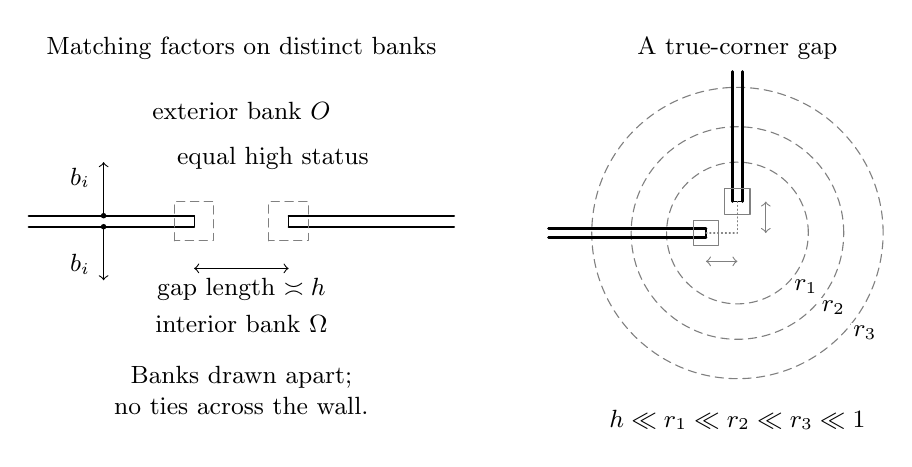
\begin{tikzpicture}[x=1cm,y=1cm,font=\small,line cap=round,line join=round]
  \node[align=center] at (2.7,4.5) {Matching factors on distinct banks};
  \node at (2.7,3.7) {exterior bank $O$};
  \node at (2.7,1.0) {interior bank $\Omega$};
  \foreach \y in {2.23,2.37} {
    \draw[line width=.8pt] (0,\y) -- (2.1,\y);
    \draw[line width=.8pt] (3.3,\y) -- (5.4,\y);
  }
  \draw (2.1,2.23) -- (2.1,2.37);
  \draw (3.3,2.23) -- (3.3,2.37);
  \draw[gray,densely dashed] (1.85,2.05) rectangle (2.35,2.55);
  \draw[gray,densely dashed] (3.05,2.05) rectangle (3.55,2.55);
  \fill (.95,2.37) circle (.035);
  \fill (.95,2.23) circle (.035);
  \draw[->] (.95,2.4) -- (.95,3.05);
  \draw[->] (.95,2.2) -- (.95,1.55);
  \node[left] at (.9,2.85) {$b_i$};
  \node[left] at (.9,1.75) {$b_i$};
  \node at (3.1,3.1) {equal high status};
  \draw[<->] (2.1,1.7) -- (3.3,1.7);
  \node[below] at (2.7,1.7) {gap length $\asymp h$};
  \node[align=center] at (2.7,.15)
    {Banks drawn apart;\\no ties across the wall.};
  \begin{scope}[shift={(9,2.15)}]
    \foreach \radius in {.9,1.35,1.85} {
      \draw[gray,densely dashed] (0,0) circle (\radius);
    }
    \draw[line width=1pt] (-2.4,.06) -- (-.4,.06);
    \draw[line width=1pt] (-2.4,-.06) -- (-.4,-.06);
    \draw[line width=1pt] (-.06,.4) -- (-.06,2.05);
    \draw[line width=1pt] (.06,.4) -- (.06,2.05);
    \draw (-.4,-.06) -- (-.4,.06);
    \draw (-.06,.4) -- (.06,.4);
    \draw[gray,densely dotted] (-.4,0) -- (0,0) -- (0,.4);
    \draw[gray] (-.56,-.16) rectangle (-.24,.16);
    \draw[gray] (-.16,.24) rectangle (.16,.56);
    \node[below right,fill=white,inner sep=1pt] at (.68,-.55) {$r_1$};
    \node[below right,fill=white,inner sep=1pt] at (1.03,-.82) {$r_2$};
    \node[below right,fill=white,inner sep=1pt] at (1.43,-1.14) {$r_3$};
    \draw[<->,gray] (-.4,-.36) -- (0,-.36);
    \draw[<->,gray] (.36,0) -- (.36,.4);
    \node[align=center] at (0,2.35) {A true-corner gap};
    \node[below] at (0,-2.12) {$h\ll r_1\ll r_2\ll r_3\ll1$};
  \end{scope}
\end{tikzpicture}
\caption{Paired walls and the local geometry of gap closure. Each surviving wall has distinct interior and exterior bank incidences, opposite wire designations, and matching factors $b_i$ evaluated with their own normals. Opening a straight gap produces two separately buffered tips; at a true corner, comparable lengths are removed on both incident sides. The dotted corner records where the filled wall would lie and supplies no connection or boundary segment for a Jordan closure. The nested radii satisfy $h\ll r_1\ll r_2\ll r_3\ll1$, with the mesh limit taken before gap closure. All geometry is schematic.}
\label{fig:paired-walls}
\end{figure}


\begin{remark}[Positive normalization and passage errors]
\label{obs:normalization}
For any positive $A$, writing $\nu_A=A\mu/\EE_\mu A$ gives the exact
identity
\[
 \frac{\EE_\mu\mathcal O}{\EE_\mu A}
       =\EE_{\nu_A}(\mathcal O/A).
\]
Consequently an exceptional event is discarded under the tilted law,
using moments of $\mathcal O/A$; its unweighted probability alone
does not control a normalized signed tensor.

We will also use the following elementary quantitative form.  Suppose
$Y_n\ge0$, $\EE Y_n\ge C^{-1}n^{-a}$,
$\EE Y_n^2\le Cn^a$, and $X_n\ge0$ has bounded exponential moments
at every fixed rate.  Then for fixed $K\ge1$ and every $\eta>0$,
\begin{equation}
 C_\eta^{-1}n^{-\eta}
 \le\frac{\EE[Y_nK^{\pm X_n}]}{\EE Y_n}
 \le C_\eta n^\eta.
 \label{obs:absorb-passages}
\end{equation}
Indeed, split at $X_n=\delta\log n$, with
$\delta\log K<\eta$.  On this event the extra factor has the desired
bounds.  Cauchy--Schwarz and an exponential moment of sufficiently
large fixed rate make both tail expectations, with or without
$K^{X_n}$, smaller than any prescribed inverse power of $n$.
Choose that power larger than $a+1$ and divide by $\EE Y_n$.
Increasing $C_\eta$ covers bounded $n$.  The positive local factors
used below have the required polynomial bounds by
Proposition~\ref{prop:tilts}; this is the precise meaning of an
$o(\log n)$ passage allowance.
\end{remark}

\begin{lemma}[Separated surface partitions]
\label{lem:obs-surface}
Let finitely many straight finite wall fragments have fixed shapes
and positive mutual separation.  Complete each as an isolated
positive slit, with boundedly many wire changes.  If $Z_s$ is its
partition relative to the plane vacuum and $Z_{\rm all}$ is the
partition with all these slits, then
\begin{equation}
 Z_{\rm all}\asymp\prod_s Z_s,
 \label{obs:surface-product}
\end{equation}
uniformly in the mesh.  Reversing all cap-wire polarities on both
banks of one straight slit changes $Z_s$ by a bounded factor.
The same holds under a lattice symmetry with cap data transported
and color names exchanged when necessary.

Positive local nest or straddle factors in separated buffered patches
can also be compared in products under these completed-slit laws.
In particular, the baseline tip and flat-change expectations in a
correct expansion and in its reflected complementary convention
are comparable when their local counts and weights are transported
by that reflection.  Constants may depend on the fixed slit geometry
and the chosen positive weights.
\end{lemma}

\begin{proof}
Enclose each fragment in its own patch, with a vacant bulk collar
and a further disjoint buffer.  Let $X_s$ count passages through that
collar.  Compare the actual incremental loop change $\Delta\ell_s$
of the surgery with $\Delta\ell_s^\circ$, calculated after closing
the patch ports by the same arbitrary pairing before and after
surgery.  A strand end whose continuation is not determined inside
the patch must first traverse the collar.  There are $O(X_s)$ such
ends; changing their pairing changes either completed cycle count
by at most their number.  Therefore
\[
 |\Delta\ell_s-\Delta\ell_s^\circ|\le C X_s,
\]
including when other surgeries have already been performed outside.
For a fixed sufficiently large $K$, simultaneous truncation
$X_s\le K$ has probability bounded below under the law with all
completed slits, by Proposition~\ref{prop:passage-moments}.
On that event all actual surgery weights and their local versions
are comparable.  With
$G_s=d^{\Delta\ell_s^\circ}\one_{\{X_s\le K\}}$, it follows that
\[
 Z_{\rm all}\asymp\EE_0\prod_sG_s,
 \qquad Z_s\asymp\EE_0G_s.
\]
The bounded collar comparison of Lemma~\ref{disk:initial-collars},
applied successively across the disjoint collars to these nonnegative
local functions, compares the first expectation with the product
of the others.  This proves \eqref{obs:surface-product}.

Translate an isolated straight fragment by one tile step tangent
to itself.  Plane invariance, with color exchange if required,
preserves its partition.  The translated caps agree with the
reversed caps except at a bounded number of ports near tips and
changes.  The remaining pairings differ on only that many ends,
so their completed loop counts differ by a bounded number.  Since
$d>0$ is fixed, the ratio of partitions is bounded above and below.
The same argument after a lattice symmetry proves its stated form.
This compares partitions, and makes no pointwise density assertion
for changing every cap along a long wall.

Finally condition successively outside the separated local buffers.
The bounded collar densities of Lemmas~\ref{disk:initial-collars}
and~\ref{disk:thin-collars} compare the expectations of arbitrary
nonnegative functions supported on their smaller patches, so they
apply to the positive powers of the indicated counts.  Reflection
across a ray exchanges its two banks and wires; reflection at a flat
change exchanges its two assignments.  Local factors on opposite
banks use disjoint half-sector buffers up to the intact wall and
are compared separately.  These charts contain only the fixed
adjacent bank portions, so all their named classes, including
partial intervals, have a fixed bound.  Reducing a cutoff by a fixed
factor when needed costs a bounded ratio by Proposition~\ref{prop:tilts}.
This proves the last assertion without identifying the two global
cap laws pointwise.
\end{proof}

\subsubsection{Inversion and the exterior phase}
On a complete wall, slide the short strings onto their bank.  The
resulting raw profile is
\[
 H_R-\tfrac12+P_R=H_R^I+H_D-\tfrac12-H_D^I,
\]
so it differs from the ideal profile by one constant.  A constant
shift cancels on an unmarked arc; with one outward source it produces
one fixed phase.  Use inversion $\iota(\zeta)=1/(\zeta-z_*)$ and a
continuous lift
$\psi=\arg\iota'$ off the chosen cut.  The inverted normal is
$\theta_O+\psi$.  On the clockwise exterior lap $\psi$ increases by
$4\pi$, making its total normal turn $2\pi$.  For an oriented
drawn arc with signed cut-intersection number $I$, its image turn is
\begin{equation}
 W^I=W+\psi(\mathrm{end})-\psi(\mathrm{start})-4\pi I.
 \label{obs:inversion-turn}
\end{equation}
The boundary normal factors cancel the endpoint terms.  At a marked
arc the two pieces have additional start terms, canceled by the
change of the source tangent gauge $e^{\ii\rho\alpha}$.
Prefix intersections are unchanged topologically.  The total
charge $-2$ along the unsplit cut supplies exactly the remaining
multiplier from $-4\pi I$ in the winding phase.  This proves that
every bounded open arc before the first splitting scale has its
ideal inverted-disk weight, up to the common source phase.  Only
turn lifts and intersections were used; the exterior probability
law has not been transformed by conformal invariance.

For the source profile, let $H^I_{V^I(u)}$ be the $c_*$-removed
tree polynomial \eqref{obs:H} for the ideal four-change profile in
the inverted coordinates on $O\cup\{\infty\}$.  Its tree is formed
from the physically sampled exterior boundary arcs, and its root
is the exterior gap at $p$.  Define
\begin{equation}
 J_n(u)=
 \frac{\EE_{\mu_{\rm ext,open}}H^I_{V^I(u)}}{P_0G_0}.
 \label{obs:exterior-observable}
\end{equation}
The law here is exactly \eqref{obs:exterior-open-law}; it has not
been conformally transformed.  The common inversion phase is not
part of $J_n$.  Its raw boundary arcs form a finite tree almost
surely by Proposition~\ref{prop:plane-limit}; no tiles at infinity
are needed.  The same finite tree bounds as in the interior and
Propositions~\ref{prop:passage-moments} and~\ref{prop:screens}
give local boundedness and equicontinuity in the reserved strip.
Indeed a nonlocal arc has a fixed-scale passage near the bounded
wall, whereas separating two nearby probe points requires an arm
from their vicinity to that wall.  At $p$ and $d_0$, local two-color
screens give the corresponding tree boundary values: the value at
$p$ tends to zero, while at the second exterior mark $d_0$ the
normalized value differs by $o(1)$ in the same ordered limit from
the expectation of
$\one_{E^I}+d\one_{(E^I)^c}$, where $E^I$ is the first exterior
designation's opposite-interval connection.  That expectation lies
in $[d,1]$.
Thus every locally uniform limit $J$ is continuous and
nonconstant on this connected strip.

For the unmarked profile the ideal open-arc weights are strictly
positive.  One and three changes give $w(1/4)=w(3/4)$; two changes
give $\sin(3\lambda/2)/\sin\lambda$; zero or all four give the
ordinary staggered cap weights.  The local drop is $1/4$ also at
$p$: the physical exterior base increases by $1$ on a second lap,
and the launches of total charge $-2$ supply the missing shift.
The wrong local drop is $-1/4$.  These shifts are unchanged by
gaps away from the marks.  Cap elimination, first inside the four
cutoffs and then at a fixed small wall scale, therefore gives for
the ideal arc product $A^I$, divided by deterministic cap loops,
\begin{equation}
 C^{-(1+X_0)}\le A^I/V_{\rm wt}\le C^{1+X_0},
 \label{obs:ideal-positive}
\end{equation}
where $X_0$ has bounded exponential moments at every fixed rate,
also under the displayed local tilts.  In particular its normalized
positive expectation is bounded above and below.

\begin{lemma}[Distant signed normalization]
\label{lem:obs-distant}
For a closed exterior raw loop $\gamma$, let
$A_\gamma=\sum_{w_j\text{ inside }\gamma}a_j$, where inside is
its physically bounded side, and set
\begin{equation}
 y_\gamma=
 \begin{cases}
 \cos((A_\gamma-1)\lambda)/\cos\lambda,
       &\gamma\text{ surrounds the wall},\\
 \cos((1+A_\gamma)\lambda)/\cos\lambda,
       &\gamma\text{ does not surround the wall}.
 \end{cases}
 \qquad Y=\prod_\gamma y_\gamma.
 \label{obs:closed-loop-ratios}
\end{equation}
These are exactly the changed closed-loop ratios in either exterior
construction.  For sufficiently large fixed $L$, under the positive
exterior law $\nu\propto U\mu_{\rm ext}$, or
$\nu\propto UV_{\rm wt}\mu_{\rm ext}$, one has
\begin{equation}
 \EE_\nu(Y/U)\ge c_L>0,
 \qquad \EE_\nu|Y/U|^p\le C_{p,L}\quad(p>0).
 \label{obs:distant-bounds}
\end{equation}
The bounds are uniform in large $R_0$ and fine mesh, and hold with
the same type of constants after conditioning in separated
near-wall patches away from the endpoint buffers.
\end{lemma}

\begin{proof}
Sum the two loop orientations and count counterclockwise string
intersections.  If the loop surrounds the wall, it surrounds all
launches and its charge contribution is $2-A_\gamma$; otherwise
it surrounds only the indicated endpoints.  This gives
\eqref{obs:closed-loop-ratios}.  A closed loop cannot separate the
marker of a nonzero source term from the connected wall: that
marker lies on an open arc to the wall.  Consequently source
prefixes make no additional closed-loop ratios, even when open
arcs go far.  Loops surrounding the wall with endpoint mass $0$
or $2$ have ratio $1$, and loops surrounding no insertion are
unchanged.  Only finitely many ratios are nontrivial at each mesh.

Choose a fixed large geometric constant $K$.  In corridor $j$,
between radii $Kr_j$ and $r_{j+1}/K$, every winding loop encloses
exactly the first $j$ endpoints.  Write $M_j$ for its product of
ratios, and $M=\prod_jM_j$.  For $0\le A\le2$,
\[
 1\le v(A):=\frac{\cos((A-1)\lambda)}{\cos\lambda}
       \le(\cos\lambda)^{-1},
\]
so every $M_j\ge1$.  Besides the local nests in $U$ and these
corridor loops, every nontrivial loop has a passage in one of
finitely many fixed-ratio endpoint bands.  A loop excluding $z_*$
and enclosing an endpoint outside its cutoff separates that
endpoint from $z_*$ and has such a passage.  A winding loop with
an intermediate endpoint mass either lies in its corridor or
meets a bounding band.  Fixed box and shell covers, with the
tilt-edge bounds of Proposition~\ref{prop:tilts}, therefore give
a count $X$ such that, for each fixed $t$,
\begin{equation}
 \EE_\nu e^{tX}\le C_t,
 \qquad |Y/U|\le MC^X,
 \qquad Y/U\ge MC^{-X}\ \text{on }\mathcal B^c.
 \label{obs:distant-sandwich}
\end{equation}
Here $\mathcal B$ is the event that a loop excluding $z_*$ encloses
at least two endpoints.  Off this event all nonlocal ratios other
than the corridor factors belong to a fixed finite positive set:
an excluded-wall loop contains at most one small charge, to which
\eqref{obs:small-charges} applies.  The constants in the exponential
bound are independent of $R_0$ and sufficiently large $L$.

Every winding loop in a corridor traverses one of $O(\log L)$
dyadic passage bands.  Color their disjoint buffers with a fixed
number of colors, apply the conditional passage moment bound in
one color successively, and use H\"older across colors.  Their
supports avoid the endpoint tilts.  Thus, for each fixed $b>0$,
\begin{equation}
 \EE_\nu M^b\le C_bL^{A_b}.
 \label{obs:corridor-moments}
\end{equation}

If a bad loop has smallest enclosed endpoint index $j$, it crosses
corridor $j$ radially.  It cannot cross any raw winding loop there,
so $M_j=1$ on this event, denoted $\mathcal B_j$.  Successive actual
circuit screens in that corridor, conditioned on all endpoint
patches and the other corridors, give
\[
 \PP_\nu(\mathcal B_j\mid\mathcal G_j)\le CL^{-\alpha},
\]
where $\mathcal G_j$ includes the variables $M_i$, $i\ne j$.
This uses only the conditional screen bounds of
Proposition~\ref{prop:screens}; the held data impose permitted
radial cap partitions on the fresh annuli, which have no bank hubs.
With $m=\EE_\nu M\ge1$ and
$M^{(j)}=\prod_{i\ne j}M_i$, we obtain the relative estimate
\begin{equation}
 \EE_\nu[M\one_{\mathcal B}]
 \le\sum_j\EE_\nu[M^{(j)}
            \PP_\nu(\mathcal B_j\mid\mathcal G_j)]
 \le C L^{-\alpha}m.
 \label{obs:bad-before-passages}
\end{equation}

For completeness, the passage factor preserves a strict relative
power.  Set $c=\log C$ and choose $\vartheta>0$ with
$c\vartheta<\alpha/2$.  Splitting at $X=\vartheta\log L$ gives
\[
 \EE_\nu[MC^X\one_{\mathcal B}]
 \le C L^{-\alpha+c\vartheta}m
   +(\EE_\nu M^2)^{1/2}
     (\EE_\nu[e^{2cX};X>\vartheta\log L])^{1/2}.
\]
For $t>2c$ the last term is at most
$C_tL^{A_2/2-(t-2c)\vartheta/2}$.  Choose the fixed rate $t$
so large that this exponent is below $-\alpha/2$, and use $m\ge1$.
It follows that
\begin{equation}
 \EE_\nu[MC^X\one_{\mathcal B}]
       \le C'L^{-\alpha/2}m.
 \label{obs:relative-signed-error}
\end{equation}
Likewise, for every $\eta>0$, split at
$X=(\eta/c)\log L+H$ if $c>0$.  Cauchy--Schwarz,
\eqref{obs:corridor-moments}, and an exponential moment with rate
$t>cA_2/\eta$ make the $M$-weighted tail at most $m/2$, by taking
the fixed $H$ large.  Hence
\begin{equation}
 \EE_\nu[MC^{-X}]\ge c_\eta L^{-\eta}m.
 \label{obs:positive-relative-mass}
\end{equation}
For $C=1$ these conclusions are immediate.  Equations
\eqref{obs:distant-sandwich}, \eqref{obs:relative-signed-error}
and \eqref{obs:positive-relative-mass}, with $\eta<\alpha/2$,
give
\[
 \EE_\nu(Y/U)
 \ge\bigl(c_\eta L^{-\eta}-2C'L^{-\alpha/2}\bigr)m>0
\]
once $L$ is sufficiently large.  This proves the uniform positive
lower bound.  All fixed absolute moments follow from
$|Y/U|\le MC^X$, \eqref{obs:corridor-moments}, and H\"older.
The arguments used conditional passage and screen estimates in
buffers separated from the near-wall patches, so the claimed
conditional uniformity follows as well.
\end{proof}

\subsubsection{Source bounds and complete-wall factorization}
We record an absolute bound which will also be needed on exceptional
gapped configurations.  Write each pure string starting at $p$ as a
short connector along the exterior bank toward its non-probe side,
followed by the rest of the string.  Retain the connector's diagonal
matrices in the bank factors, in the original lane order.  Deform only
the remaining path, with its endpoints fixed, by
Lemma~\ref{lem:current-identity}.  This expresses a small displacement
of the continuing route while retaining every crossed-port phase and
the charge at its original endpoint $p$.
Each source can now be put in a regular simple tube with $p$ in
the relative interior of a flat entrance, clear on both sides,
and the target deep inside.  Other tube sides avoid walls,
strings, and the other tube.  Finitely many such choices cover
compact probe sets.

For a fixed pairing minimize crossings of the disjoint raw crosscuts
separating the entrance from the target.  A small separating crosscut
near the entrance cuts off $p$, since it cannot contain the deep
target.  The solid entrance makes it an entire local launch arch,
not a short return of a larger strand.  All other relevant open
crosscuts have macroscopic tube subpassages; repeated visits of one
strand give disjoint such passages.  A tiny separator at the deep
target is a closed loop and cannot carry a nonzero outward source
marker.  The two outward markers cannot lie on one raw arc or on a
closed loop, since its orientation cannot supply two outward ends.

After including the short and distant charges, the local unpassed
drop at either launch is $-s$.  It has weight zero.  Passing its
source prefix changes it to $-s-1$, with the $Q^{-1}$ sign, giving
unit absolute weight.  Thus only the last nested launch arch can
be marked in a nonzero term.  The other local changes $s,t,s$ have
unit weights.  Ordinary small disks cancel their caps by the
finite elimination in Lemma~\ref{physical:cap-elimination}; a
geometric corner without a wire change has zero-drop staggering.
Every remaining choice costs at most a constant per macroscopic
passage.  Thus for a complete wall the absolute source sum divided
by its deterministic loops and by $U$ is bounded by
\begin{equation}
 |Y/U|C^{1+X_0},
 \label{obs:absolute-source-bound}
\end{equation}
with all fixed exponential moments for $X_0$ under the relevant
tilts.  The analogous diagonal bound has the factors $U_z$ and
$V_{\rm wt}$ removed.  Near $z$ the full diagonal changes the loop
weight to $-2$, whose absolute ratio is $2/d$; beyond its cutoff
every enclosing loop has a fixed-scale passage.  Its local
interior changes have unit magnitude, including the exiting
prefix at $p$.  The exterior local changes are exactly the
$V_{\rm wt}$ factors.  These observations prove all fixed
absolute moment bounds for both normalized integrands.

The next factorization keeps the wall complete.  Independence of the
interior and exterior positive laws is exact; the source error comes
from sending the exterior string-splitting scales to infinity.
After this reduction we will compare gapped walls with the complete
wall using the same positive normalizations.

\begin{proposition}[Complete-wall factorization]
\label{prop:obs-factorization}
For the source tensor there are numbers $a_n(R_0,L)$ independent
of both probes, with $c_L\le|a_n|\le C_L$, such that
\begin{equation}
 \begin{aligned}
 \mathcal H_f(z,u)&=a_n(R_0,L)h_n(z)J_n(u)+e_n(z,u;R_0,L),\\
 \lim_{R_0\to\infty}\limsup_{n\to\infty}
       \sup_{(z,u)\in K}|e_n|&=0
 \end{aligned}
 \label{obs:source-factorization}
\end{equation}
for each compact probe set $K$, with sufficiently large fixed $L$.
Every locally uniform subsequential limit of $J_n$ on the reserved
strip is continuous and nonconstant.

For the diagonal tensor, write $\mu_{\rm in}$ for the interior
deterministic-cap law, $R_*=d^{\ell_{\rm open}-\ell_{\rm det}}$,
and $N(z)$ for all closed interior raw loops surrounding $z$.
There is a probe-independent exterior scalar $a_n^I(R_0,L)$ such
that the exact full-wall identity is
\begin{equation}
 \mathcal R_f(z)=a_n^I(R_0,L)
 \frac{\EE_{\mu_{\rm in}}
   [R_*\sigma(\operatorname{col}(V(z)))D_{V(z)}(2/d)^{N(z)}]}
 {\EE_{\mu_{\rm in}}U_z}.
 \label{obs:diagonal-factorization}
\end{equation}
For sufficiently large fixed $L$,
\begin{equation}
 \liminf_{R_0\to\infty}\liminf_{n\to\infty}|a_n^I|>0,
 \qquad \limsup_{R_0\to\infty}\limsup_{n\to\infty}|a_n^I|<\infty.
 \label{obs:diagonal-exterior-nonzero}
\end{equation}
No convergence of either scalar is required.
\end{proposition}

\begin{proof}
On a complete wall the two positive capped laws are independent:
their raw pairings and separate cap disks share no connection.
For the source tensor the interior factor is $h_n$ times
$c_*P_0G_0$ and the open-to-deterministic partition ratio.  That
ratio is bounded above and below, because only the four unmatched
ports are re-paired.  The diagonal finite tree expansion gives the
interior factor in \eqref{obs:diagonal-factorization}, with the
parity factor already fixed in \eqref{obs:residual-normalization}.
This proves the exact assertion once $a_n^I$ is defined as the
normalized exterior expectation.

Actual circuits between the bounded wall and the first endpoint
scale make the probability of a boundary raw arc reaching that
scale tend to zero, also under $U$ and $UV_{\rm wt}$ tilts.
On its complement the inversion calculation is exact.  The
moment bounds in Lemma~\ref{lem:obs-distant},
\eqref{obs:ideal-positive}, and
\eqref{obs:absolute-source-bound} make the exceptional contribution
$o(1)$ by H\"older, in the stated order of limits.

Choose $1\ll R_1\ll R_2\ll R_0$ with all successive ratios
diverging.  Truncate the ideal arc factor to zero unless all its
boundary arcs stay inside $R_1$.  It is then readable inside that
radius.  Similarly $Y/U$ is readable outside $R_2$ except when a
raw path joins that radius to an endpoint band: loops created
entirely at the smaller scales have ratio $1$.  Screening makes
both exceptions rare, and the same moments control the product
errors.  The inward relative bulk comparison in
Proposition~\ref{prop:relative-collars} factors the expectations
of the two truncated factors with error $o(1)$.  These collars are
vacant full annuli with no named bank hubs.  To see that it
applies to a signed factor, apply the uniform relative density
bound to its positive and negative real and imaginary parts;
their absolute expectations are bounded by the moment estimates.
The same comparison applied to absolute parts removes the remote
tilt from the near factor.  With $V_{\rm wt}$ present it retains
exactly that near-wall tilt and removes only $U$.

In the source case the near expectation is the normalized ideal
tree observable $J_n$, times its fixed nonzero tree and cap
normalizers.  The far expectation is $\EE_\nu(Y/U)$, bounded
above and away from zero by Lemma~\ref{lem:obs-distant}.
Absorb these constants and the common inversion phase into
$a_n$.  This proves \eqref{obs:source-factorization} and its
uniformity; the assertion about $J_n$ was proved above.
In the unmarked case the near expectation is positive and
bounded above and below by \eqref{obs:ideal-positive}.  Its
product with the positive distant expectation gives
\eqref{obs:diagonal-exterior-nonzero}, including the harmless
common phase.  At no stage is a lower bound for a signed interior
observable used.
\end{proof}

\subsection{Closing wall gaps after positive normalization}
\label{obs:closing-gaps}

\begin{proposition}[Common gap closure]
\label{prop:obs-gap-closure}
Fix the distant strings, their locations, and all other geometric
features.  Open finitely many separated gaps of lengths comparable
to $h$, away from marks and insertion corridors; at a true corner
remove comparable intervals on both sides.  Let $g$ be this wall
and let $f$ fill these gaps, possibly retaining other fixed gaps.
For the tips being filled, take cutoff radii at one fixed positive
fraction of $h$, with buffers clear of the other features for all
small $h$.  Keep the endpoint factor $U$ and all retained cutoff
patches fixed during this closure.  Constants below may depend on
that fixed cutoff fraction.
For the source normalization there are positive numbers $b_n$
independent of $z,u$, with $c\le b_n\le C$, such that
\begin{equation}
 \mathcal H_g(z,u)=b_n\mathcal H_f(z,u)+e_{n,h}(z,u),
 \qquad
 \lim_{h\downarrow0}\limsup_{n\to\infty}
       \sup_{(z,u)\in K}|e_{n,h}|=0.
 \label{obs:source-gap-closure}
\end{equation}
For every fixed interior $z$, the same assertion holds for
$\mathcal R_g(z)$ and $\mathcal R_f(z)$, with a positive bounded
factor $b_n(z)$.  Constants may depend on the fixed remaining
features and on $K$ or $z$.  In particular, a smaller second
collection of gaps can be closed before the first.
\end{proposition}

\begin{proof}
We use the same tile pairings in both cut conventions.  A raw arc
or port interaction is affected if it uses a newly missing port;
the gapped diagram joins the filled raw paths which end there.
For the source case set $S=UT_f$, and for the diagonal case set
$S=U_zUV_{\rm wt}T_f$.  Put $T=T_g/T_f$ and
\begin{equation}
 \nu_g=\frac{ST\mu_g}{\EE_{\mu_g}(ST)},\qquad
 \nu_f=\frac{S\mu_f}{\EE_{\mu_f}S}.
 \label{obs:gap-tilted-laws}
\end{equation}
All factors of $S$ are supported away from the gaps being filled.
Our goal is to separate the normalized diagram into a positive local
multiplier near the gaps and a common signed factor away from them.
The separation is exact on a screening event.  Uniform moments under
both tilted laws will control its complement before the relative
collar comparison factors the two expectations.

\paragraph{The local positive multiplier.}
Choose $h\ll r_1\ll1$.  In the common collars impose an actual
primal screen between the wall rays in the sector carrying primal
wire portions, and an actual dual screen in the other sector,
which has no bank or hub attachment.  The only bank attachments in
the first sector are the two continuous primal ray portions, each
crossing the collar and met by its primal screen.  The sectors have
no direct contact inside the collar.  By testing many separated
shells outside the tip supports, Proposition~\ref{prop:screens}
and the tilt bounds make this event, called $G_{\rm in}$, have
probability tending to one under $\nu_g$, uniformly given remote
data and deeper tip data.  It confines every affected path to the
$r_1$ patches.  The induced outer primal ties are the same in the
two conventions: any connection through a deeper patch enters
the already connected primal screen, also if it bypasses through
one of the wire portions joined by that screen.  Represent those
wires by deterministic connections along the designated intervals.
Euler's formula then makes $\ell_f-\ell_g$ a difference of local
component counts plus deterministic constants.  This conclusion
may first be read with all exterior edges fixed.

There is therefore a local factor $B$ such that, on $G_{\rm in}$,
\begin{equation}
 \mathcal O_g=B\mathcal O_f.
 \label{obs:gap-local-equality}
\end{equation}
This is an identity of the summed diagram expressions, including
when their common exterior factor vanishes: $B$ is formed from
the affected local spin weights and $d^{\ell_f-\ell_g}$, not by
dividing a possibly zero observable.  It is strictly positive.
Indeed the patch is a disk with two radial notches ending at its
separated tips.  A same-bank simple arc, including one threading
the gap, has opposite high statuses at its ends and the ordinary
staggered $d,1$ weights.  For an opposite-bank arc oriented from
the interior port $i$ to the exterior port $j$, high statuses
agree and the endpoint directions are the two interior normals.
The matching factors and the winding formula of
Lemma~\ref{physical:winding} give its orientation sum as
\begin{equation}
 \frac{\cos\{\rho(W+\theta_i-\theta_j)/2\}}{\sin\lambda}.
 \label{obs:opposite-bank-amplitude}
\end{equation}
The lifted turn $W+\theta_i-\theta_j$ is $\pm2\pi$ around one
ray tip, and $0$ across the slot between the two rays.  Thus the
two weights are respectively $\cot\lambda$ and $1/\sin\lambda$,
both positive.  To verify the lift, round the boundary-attached
notches and separate their bank incidences.  The resulting region
is a topological disk, and an affected raw arc is a proper embedded
crosscut: an intermediate bank contact would terminate that raw
arc, while confinement keeps it off the outer patch boundary.
Crosscuts with the same endpoint incidences are ambient-isotopic
relative to this disk boundary.  The isotopy can be fixed in short
endpoint collars, so the endpoint tangents and normal lifts stay
fixed and the integer turn defect cannot change.  For collinear
rays, a representative around a single ray tip has defect
$\pm2\pi$, and a representative across the slot between different
rays has defect $0$.  Any Jordan closure used here follows the
rounded disk boundary, not the virtual filled wall through the
slot.  In particular the other notch, which is attached to the
outer boundary, cannot be enclosed by a same-ray crosscut and its
short bank closure without a crossing.  Bending one ray through
the corner angle rotates its endpoint normal and tangent equally,
preserving the defect.  Newly closed
internal loops have weight $d>0$.  These observations prove
positivity of every local factor in $B$.

There is a fixed $K$ and a count $X_h$ with all fixed exponential
moments under $\nu_g$ such that
\begin{equation}
 K^{-(1+X_h)}\le B/T\le K^{1+X_h}
       \quad\hbox{on }G_{\rm in}.
 \label{obs:gap-local-bounds}
\end{equation}
Here is why the count has no accumulation over intermediate
scales.  In both cut conventions remove affected boundary arcs
of diameter below a small fixed fraction of $h$, together with
their disk descendants, starting with innermost arcs.  In $f$
they lie on homogeneous continuous intervals, including the
newly filled positions.  In $g$ each such disk lies against one
bank or across one tip change.  Its disk is also short by the
straight or single-corner geometry, and cannot span both tips.
Remove any common unaffected descendants needed by either
elimination as well.  They have ends on a common bank piece
and the same neutral disk and intervening arcs, so their union
is an admissible common removal.

The high-low zero-change removal creates one cap loop and cancels
its $d$ weight; the low-high removal transports the cap pattern
with weight $1$.  Across one tip both statuses agree, one unmatched
port is transported, and no loop is created, leaving exactly
$\cot\lambda$.  No whole interval is erased.  The number of
these removed tip arches differs from $N_{\rm tip}$ by $O(X_h)$:
any disagreement meets the edge of its cutoff and has a slot-scale
passage.  Every surviving affected boundary arc also has a
slot-scale passage.  Filled paths are disjoint segments of the
gapped paths, so they obey the same count.  Bulk, straight-wall,
and tip buffers, including cutoff-edge buffers, give all fixed
exponential moments by Propositions~\ref{prop:passage-moments}
and~\ref{prop:tilts}.

On every surviving common solid interval, both residual caps pair
adjacent high-low ports.  Only interval ends and noncommon survivors
interrupt them, at $O(1+X_h)$ ports.  Their remaining loop counts
differ by at most this number, whatever the distant ties are.
New local closed loops cancel their ordinary spin weights.  This
proves \eqref{obs:gap-local-bounds} while retaining the exact
positivity.

\paragraph{Moments on all configurations.}
For every fixed $p>0$, the variables
$\mathcal O_g/(ST)$ and $\mathcal O_f/S$ have bounded absolute
$p$-moments under $\nu_g$, uniformly as $h\downarrow0$; the
second has the same bound under $\nu_f$.  These bounds hold
without $G_{\rm in}$.  To prove this, make the short removals just
described regardless of how far the affected surviving paths
travel.  Short affected loops and disks avoid every insertion,
and are neutral except for their removed tip factors.  Non-short
affected arcs cost at most $K^{X_h}$, including the interruptions
they make in residual caps.

Eliminate remaining filled neutral disks up to a fixed small
macroscopic threshold, chosen below the separations of retained
gaps and other features.  This includes all intermediate straddles
at the newly filled homogeneous locations.  Common ordinary disks
cancel caps.  Retained tips yield their factors in $T_f$, up to
fixed-scale cutoff-edge passages.  The source tubes and launch
calculation preceding Proposition~\ref{prop:obs-factorization}
hold unchanged with remote gaps, since their solid entrances
are unchanged.  There are only passage-counted nonlocal marker
choices.  For the diagonal tensor the local interior changes have
unit magnitude, the exterior changes yield $V_{\rm wt}$, and
the local loops at $z$ yield $U_z$.  The distant endpoint nests
yield $U$ in either case.  A loop outside these patches that
separates a source marker from its start must also cut off an end
of its open arc on a solid of length bounded below; it cannot be
tiny.  Other strings have only their specified endpoint and bank
charges.  Loops enclosing all finite data have ordinary ratio $1$.
Consequently, with the distant geometry held fixed,
\begin{equation}
 |\mathcal O_g/(ST)|+|\mathcal O_f/S|
       \le K^{1+X_0+X_h}.
 \label{obs:gap-absolute-moments}
\end{equation}
The constant may depend on that geometry.  The count $X_0$ uses
only its fixed scales and has all fixed exponential moments.
A path of fixed diameter near a shrinking slot has a fixed-size
subpassage outside a small neighborhood of the slot; the usual
bulk or sector buffers count it even when the wall is newly
open.  Again the filled paths are disjoint raw segments.  Thus
Propositions~\ref{prop:passage-moments} and~\ref{prop:tilts}
prove the stated bounds under both laws.  In particular all
exceptional-event contributions tend to zero by H\"older.

\paragraph{Exterior readability and relative comparison.}
Choose $r_1\ll r_2\ll r_3\ll1$, with all ratios diverging as
$h\downarrow0$.  There is an approximation $F_{\rm out}$ to
$\mathcal O_f/S$, readable outside the $r_2$ patches, exact
unless a raw passage traverses a common collar from $r_2$ to
$r_3$; set it to zero on that exterior exceptional event.  To
verify this, vary an arbitrary inner fill while the outer data
are fixed.  In the absence of such a passage, the variation
affects only disks against homogeneous continuous intervals in
the filled convention.  Their cap elimination has net weight
$1$.  For a common elimination over all inner fills, take the
union of port blocks affected, or intervening, for some fill.
A stable arc in an intervening block pairs within it and has
the same neutral disk with its descendants.  The untouched
ports therefore inherit the same adjacent-pair reconnection
after all those blocks are deleted.  Modified internal loops
are ordinary; all source, endpoint, and remote tilt data stay
unchanged.  This proves exterior readability, not merely a
small probability of contact with the inner core.  Screens
make the exceptional event rare under both tilted laws and
\eqref{obs:gap-absolute-moments} controls its error in every
fixed smaller moment.

Define
\[
 D_{\rm in}=(B/T)\one_{G_{\rm in}}.
\]
It is nonnegative and readable inside $r_1$, with bounded fixed
moments.  Its expectation lies in $[c,C]$: the upper bound follows
from \eqref{obs:gap-local-bounds}; for the lower bound choose
a fixed cutoff $K_0$ making $\PP_{\nu_g}(X_h>K_0)<1/4$ and
then make $\PP_{\nu_g}(G_{\rm in}^c)<1/4$.  On their common
complement it is at least $K^{-(1+K_0)}$.

The outward two-sector form of
Proposition~\ref{prop:relative-collars} compares the conditional
law outside $r_2$, given an inner fill under $\nu_g$, with its
law under $\nu_f$, with relative error tending uniformly to zero.
The graph and wire representatives in the collar and beyond
are identical; only the deeper inner partition can change.  The
two screen-met continuous primal rays and the opposite sector
without bank attachments are exactly the data in the two-sector hypothesis
of that proposition.
For several patches apply this comparison successively.  Holding
the other interiors introduces only their allowed local ties,
whose external wires are still represented along the common
sides.  The factor $T$ is inside and $S$ is remote, so the same
relative estimate survives both positive tilts.  Applied to
the absolute parts of $F_{\rm out}$, its error is bounded by
the relative error times $\EE_{\nu_f}|F_{\rm out}|$.
The moment bounds and \eqref{obs:gap-local-equality} now give
\begin{align}
 \EE_{\nu_g}[\mathcal O_g/(ST)]
 &=\EE_{\nu_g}[D_{\rm in}F_{\rm out}]+o(1)\notag\\
 &=\EE_{\nu_g}D_{\rm in}\,
       \EE_{\nu_f}[\mathcal O_f/S]+o(1).
 \label{obs:normalized-gap-factorization}
\end{align}
By \eqref{obs:diagram-normalization} and
\eqref{obs:gap-tilted-laws}, these are exactly the normalized
tensors in the statement (with the same harmless parity factor
for the diagonal tensor).  Set $b_n=\EE_{\nu_g}D_{\rm in}$.
It is positive and bounded above and below.  In the source case
the law, screens, and local multiplier defining it contain no
probe positions, so it is independent of both probes and the
error is uniform on compact sets.  In the diagonal case the
$U_z$ tilt may enter its expectation; the statement uses only
each fixed $z$.  This proves both claims and the permitted
successive order of gap closures.
\end{proof}

\subsection{A normalized cancellation of the diagonal residual}
\label{obs:residual-section}

The bounded tree variables do not by themselves put the mean observable
on its four boundary lines: the line invariant contains a diagonal
term.  We now cancel that term.  The normalization in the next theorem
is essential.  In the present range the absolute weight of a wrong
bulk loop need not be at most its ordinary weight.

Fix an interior point $z$ of the polygon $\Omega$ and mesh vertices
converging to it.  Let $\mu_{\rm in}$ be its deterministic-cap law and
let $N(z)$ count all internal raw closed loops surrounding $z$.
Let $N_0(z)$ count those wholly inside the radius-$r_z$ box at $z$,
where
\begin{equation}
 r_z=\dist(z,\partial\Omega)/8,\qquad
 U_z=(2/d)^{N_0(z)}.
 \label{obs:Uz}
\end{equation}
Boxes may be taken in tile coordinates; changing their fixed shape or
radius factor changes the comparisons below only by bounded factors.
Write
\begin{equation}
 R_*=d^{\ell_{\rm open}-\ell_{\rm det}}.
 \label{obs:open-density}
\end{equation}
The two loop counts in this expression use the same switch
configuration and its open and deterministic local-cap completions.
Their difference is bounded, so $R_*$ and $R_*^{-1}$ are bounded and
$\EE_{\rm open}X=\EE_{\mu_{\rm in}}(R_*X)/\EE_{\mu_{\rm in}}R_*$.

\begin{theorem}[Normalized diagonal cancellation]
\label{thm:normalized-residual}
Let $\sigma$ have opposite signs on the two colors, each of absolute
value one.  For every fixed interior $z$,
\begin{equation}
 \frac{\EE_{\mu_{\rm in}}
  [R_*\sigma(\operatorname{col}(V(z)))D_{V(z)}(2/d)^{N(z)}]}
 {\EE_{\mu_{\rm in}}U_z}\longrightarrow0.
 \label{obs:normalized-residual}
\end{equation}
\end{theorem}

\begin{proof}
Fix sufficiently large $L$.  For every sufficiently large fixed $R_0$,
\eqref{obs:diagonal-exterior-nonzero} bounds $|a_n^I(R_0,L)|$ away
from zero for all sufficiently large $n$; the mesh threshold may
depend on $R_0$.  Restrict to this mesh tail.
By the exact factorization \eqref{obs:diagonal-factorization}, the
ratio in the theorem is $\mathcal R_f(z)/a_n^I(R_0,L)$ for our fixed
choice of $\sigma$, and its negative for the other choice.  The
parity identity \eqref{obs:parity-sign} has already converted each
enclosing-loop factor $(-2/d)$ into the signed tree factor and the
positive magnitude $2/d$.  It remains to show that $\mathcal R_f(z)$
vanishes and then use the nonzero exterior factor.

Use $\mathcal R_g$ from \eqref{obs:residual-normalization}, with the
unmarked exterior profile $H^{\rm diag}$ in
\eqref{obs:exterior-profiles} and the charge routes of
Section~\ref{obs:paired-walls}.  The two distant charge lists each
have total magnitude one and satisfy \eqref{obs:small-charges}.
Besides their endpoint factor $U$, the exterior normalization has
the flat-flip factor
\begin{equation}
 V_{\rm wt}=w(1/4)^{\sum_{\nu=1}^4N^{\rm ext}_\nu},
 \label{obs:quarter-tilt}
\end{equation}
where the four local straddle counts use disjoint buffered patches.
Open gaps of width comparable to $h$ at every true corner, away from
all these patches and from the string corridors.  The remaining solids
are separated straight fragments.  For the gapped configuration use
the tip factor $T_g$ and normalize its vacuum tensor by
\begin{equation}
 Z_g^{\rm cap}\EE_{\mu_g}[T_g S],\qquad
 S=U_z U V_{\rm wt}.
 \label{obs:residual-normalizer}
\end{equation}
All supports of $S$ remain away from the shrinking corner gaps.

\paragraph{Decay with the corner gaps fixed.}
We first show that this normalized tensor vanishes as the mesh tends
to zero at every fixed gapped geometry.  Take its absolute value using
the wrong winding expansion and complementary positive caps.
The local factors are as follows.
\begin{enumerate}[label=(\roman*),leftmargin=*]
\item Ordinary straight-bank arcs have their complementary cap weights.
At the three interior flips $p,b,d_0$ the wrong local straddle weight
is zero.  At $c$ it is $d$.  At $p$ the exiting pure prefix changes
the wrong drop to $s+1$, and $w(s+1)=0$; at the other marks the
values follow by direct substitution of $-s,-t,-s$.
\item Every exterior flat flip has correct drop $1/4$ and wrong drop
$-1/4$.  Their weights satisfy
\[
 0<w(-1/4)=\frac{\cos(3\lambda/4)}{\sin\lambda}
 \le \frac{\cos(\lambda/4)}{\sin\lambda}=w(1/4).
\]
Thus the exterior flip contribution is dominated by
\eqref{obs:quarter-tilt} and has no extra logarithmic cost.
\item A same-ray tip has magnitude $\cot\lambda$ in either expansion,
so its prescribed positive tip factor is unchanged.
\item A loop around $z$ has wrong magnitude
$2|\cos(2\lambda)|/d\le2/d$.  The loop nests wholly in its cutoff
are therefore dominated by $U_z$.  At a distant endpoint the local
ratios are $u_-(a_j)$ instead of $u_+(a_j)$.
\end{enumerate}
The facts used here are the finite winding calculation, not an
analytic continuation of a probabilistic estimate.  In particular
we have retained the factor $2/d$ at $z$.

Eliminate the short same-bank disks and their descendants with
the cap rule of Section~\ref{sec:physical}.  A remaining nonordinary
arc or loop has a passage at one of the finitely many fixed feature
scales.  Thus its absolute contribution is at most $C^{1+X}$ after
the displayed local factors, with every fixed exponential moment
of $X$ bounded by Propositions~\ref{prop:passage-moments}
and~\ref{prop:tilts}.  This also applies to each half-sector at a
paired mark: its cutoff lies on its own bank, and connections between
the two cutoff supports can only run beyond their buffers.  The
buffered collar comparison can consequently be applied successively.

The complementary and original straight-fragment cap partitions are
comparable by Lemma~\ref{lem:obs-surface}.  Reflecting across a flat
ray and using the bounded collars of Lemmas~\ref{disk:initial-collars}
and~\ref{disk:thin-collars} compares the corresponding tip
and baseline local expectations.  Consequently, relative to
\eqref{obs:residual-normalizer}, the additional upper logarithmic
cost is
\begin{equation}
 3P+D_*+\sum_{j\text{ in both lists}}
           \log\frac{F_-(a_j)}{F_+(a_j)}+o(\log n).
 \label{obs:residual-cost}
\end{equation}
Absorption of $C^{1+X}$ is legitimate at an arbitrarily small power
loss: the local factors have polynomial positive and absolute
moments, and their baselines have inverse-polynomial lower bounds.
Split at $X=\varepsilon\log n$ and use an arbitrarily large fixed
exponential-moment rate on its complement.  This supplies the
one-sided $o(\log n)$ allowance in \eqref{obs:residual-cost}.

Apply Theorem~\ref{thm:charge-budget} separately to the two lists.
The quantity in \eqref{obs:residual-cost} is at most
\[
 3P+D_*-2(P+D_*)+o(\log n)
 =P-D_*+o(\log n)
 \le-c_2\log n+o(\log n)
\]
by Lemma~\ref{lem:strict-flip}.  The normalized tensor therefore
tends to zero at each fixed collection of corner gaps.  No wrong
concave-corner factor occurs, since all solids in this estimate are
straight.

\paragraph{Restoring the polygon.}
For fixed $z$ and fixed distant geometry,
Proposition~\ref{prop:obs-gap-closure} transfers this zero limit to
the complete wall when the gaps shrink after the mesh limit.  The
normalizing supports in \eqref{obs:residual-normalizer} are remote
from the closing gaps, and the comparison multiplier is positive and
bounded above and below.  At the complete wall the interior and
exterior capped laws factor.  The interior factor is exactly
the ratio in \eqref{obs:normalized-residual}, by
\eqref{obs:diagonal-factorization}.
The unmarked exterior factor has modulus bounded away from zero
as the first distant scale tends to infinity after the mesh limit,
by Proposition~\ref{prop:obs-factorization}.  Dividing by that
factor proves the result.  The distant separation parameter is
chosen sufficiently large and then fixed throughout these limits.
\end{proof}

\begin{lemma}[Vanishing boundary residual]
\label{lem:obs-boundary-residual}
For every bounded function $\gamma$ of the two colors and every
boundary point $u$ distinct from the four marks, including an
ordinary polygon corner,
\begin{equation}
 \lim_{z\to u}\limsup_{n\to\infty}
 \left|\EE_{\rm open}
       [\gamma(\operatorname{col}(V(z)))D_{V(z)}]\right|=0.
 \label{obs:boundary-residual}
\end{equation}
The outer limit is through macroscopic interior points.
\end{lemma}

\begin{proof}
Let $R$ be the unmarked boundary interval containing $u$ and put
$g_R=1/2$ on its wire color and $g_R=-1/2$ on the other color.
Under $\mu_{\rm in}$ write the numerator integrand of
\eqref{obs:normalized-residual} as $B_*T_*$, where
\begin{equation}
 B_*=R_*\sigma(\operatorname{col}(V))
               d^{-g_R(\operatorname{col}(V))}D_V,
 \qquad
 T_*=d^{g_R(\operatorname{col}(V))}(2/d)^{N(z)}.
 \label{obs:BT}
\end{equation}
The first factor is bounded uniformly, by Lemma~\ref{lem:obs-marked}.
Choose scales
\begin{equation}
 |z-u|\ll r_1\ll r_2\ll r_3\ll1,
 \label{obs:boundary-scales}
\end{equation}
with all consecutive ratios diverging as $z\to u$, and take the
mesh limit first at every fixed choice of $z$ and these scales.

Actual screens in the regular sector at $u$ make $B_*$ measurable
outside the $r_2$ patch, except on an event whose probability tends
to zero in the scale ratios.  Use as the good event the absence of
a raw traversal of the annulus from its $r_2$ rim to its $r_3$ rim;
this event is determined by the annular diagram, hence by the
configuration outside $r_2$.  Here is the finite invariance needed
for measurability.  For every compatible filling inside $r_2$ on
this exterior event, every boundary arc affected by changing that
filling lies in one small portion of $R$ and contains no
mark in its child interval.  All marked-subtree data and the
open-to-completed pairing factor $R_*$ remain fixed.  Stable exterior
separators put the whole connected inner patch on one side or the
other.  Noncrossing therefore puts all affected on-path edges after
the stable prefix.  Their off-path factors cancel the local caps;
their on-path suffix telescopes by the ordinary-tail rule
\eqref{obs:tail}.  The sign and color factor in $B_*$ cancel
that suffix.  Define the exterior-readable truncation $B_{\rm out}$
to equal $B_*$ on this good event and zero otherwise.

Define $T_{\rm in}$ by counting only enclosing loops wholly inside
the $r_1$ patch and reconstructing the tree color from their parity
and the fixed lattice color at $z$.  This agrees with $T_*$ unless a
raw path goes from the $O(|z-u|)$ neighborhood to the $r_1$ rim:
every loop enclosing $z$ meets the segment from $z$ to a closest
boundary point.

We require errors relative to $\EE U_z$, not merely unweighted
probability errors.  Work under the positive tilt
$\nu_{U_z}\propto U_z\mu_{\rm in}$.  Its support is inside the
small box in \eqref{obs:Uz}, so separated screens outside that box
still make the exceptional events rare.  The variables
$T_*/U_z$ and $T_{\rm in}/U_z$ have uniformly bounded fixed moments.
Indeed each additional enclosing loop escapes that cutoff and meets
the short segment to a closest wall point, hence gives a passage
through a band at distance comparable to $\dist(z,\partial\Omega)$.
A bounded cover by bulk and regular-sector buffers counts these
passages.  At a corner use its sector buffer and straight-bank
buffers; when the corner is farther than that distance scale only
the straight-bank buffers are needed.  Proposition~\ref{prop:tilts}
gives the asserted moments uniformly.  Together with boundedness of
$B_*$, H\"older's inequality now gives
\begin{equation}
 \EE[B_*T_*]-\EE[B_{\rm out}T_{\rm in}]
       =o(\EE U_z),
 \qquad \EE T_{\rm in}\asymp\EE U_z.
 \label{obs:residual-truncation}
\end{equation}
For the second comparison, the truncated loop count includes $N_0$
and $2/d>1$, giving the lower bound; the same moment estimate gives
the upper bound.  The bounded positive color factor is harmless.

The inward relative sector comparison of
Proposition~\ref{prop:relative-collars}, applied between $r_1$ and
$r_2$ to the positive inner factor and the positive and negative
parts of the bounded exterior variable, yields the estimate below.
After exchanging colors if necessary, the only bank attachment is
the continuous primal interval through $u$, whose two ray portions
cross the collar and meet the same primal screen.  This is the
one-sector hypothesis of that proposition.  Thus
\begin{equation}
 \EE[B_{\rm out}T_{\rm in}]
 -\EE B_{\rm out}\,\EE T_{\rm in}=o(\EE U_z).
 \label{obs:residual-decoupling}
\end{equation}
Theorem~\ref{thm:normalized-residual}, used first at fixed $z$,
and \eqref{obs:residual-truncation}--\eqref{obs:residual-decoupling}
show that $\EE B_*$ tends to zero in the ordered limit.

Apply the same separation without a tilt to $B_*$ times any bounded
function of the tree color.  Up to a rare event, that color is read
from the inner-loop parity, whereas $B_*$ is exterior-readable.
The expectation therefore factors up to $o(1)$ into an exterior
mean tending to zero and a bounded inner mean.  Choose the color
function that reverses the extra factors in \eqref{obs:BT}, and
divide by $\EE R_*\asymp1$.  This proves
\eqref{obs:boundary-residual}.
\end{proof}

\subsection{Mixed stencils and the strict reflected cost}
\label{obs:mixed-section}

The preceding cancellation supplies the required boundary values.
We next prove holomorphicity in the interior.  Pairing an interior
stencil with an exterior one lets us use a high angular mode at one
probe and a low mode at the other; their decay powers add to two.
The strict charge budget pays the remaining reflection loss.

Call a probe pair $(z,u)$ \emph{eligible} when the following
conditions hold for the fixed initial walls, protected marks, and
distant endpoints.  Its two abscissas avoid the finitely many true
vertical wall levels.  Its ordinates avoid the horizontal wall and
feature heights and lie in disjoint open bands containing no
distant endpoint.  Writing the two probes as $(x_i,y_i)$, require
also $x_1-y_1\ne x_2-y_2$ and $x_1+y_1\ne x_2+y_2$.  All
inequalities have uniform strict margins on the compact product
neighborhoods used below.  These forbidden projections refer only
to the initial data: adaptive gap and cut locations belong to each
finite template and do not enlarge the global exceptional set.

We return to the two-source paired wall of
Proposition~\ref{prop:obs-factorization}.  The interior source runs
from $p$ to $z$ and the exterior source from $p$ to a point $u$ in
the reserved $D$-collar strip.  Its exterior ideal bases in inverted
order are $(s+1,1,s,0)$.  The interval-parallel strings set those bases;
two lists of distant charges again have total magnitude two.  At a
common starting edge the pure strings and source strings use the
ordered lanes specified in the finite path calculus.  After shrinking
the eligible probe neighborhoods, choose disjoint closed stencil boxes
inside the two source tubes.  The common diagonal routes avoid both
boxes except for each box's own arriving prefix; all pure-string
corridors avoid the boxes.  These choices are common to every local
term of the two stencils.  Normalize by
\begin{equation}
 \mathcal H_g(z,u)=
 \frac{\Xi_g(z,u)}{Z_g^{\rm cap}\EE_{\mu_g}[UT_g]}.
 \label{obs:mixed-normalization}
\end{equation}
Here $\Xi_g$ is the vacuum tensor and the denominator is positive
and independent of both probes.

For the tile-coordinate unit vectors $e_1,e_2$, we use the unscaled
two-step forward differences
\[
 \delta_j^{(2)}F(v)=F(v+2e_j/n)-F(v),\qquad j=1,2.
\]
There is no division by the step length; a subscript $z$ or $u$
specifies the probe variable.  A \emph{low stencil} is one such
two-step primitive increment.  A \emph{high stencil} compares the two
orthogonal increments with a common arriving prefix, subtracting the
second with coefficient $e^{\ii(\arg e_1-\arg e_2)}=-\ii$.
Thus $\delta_{1,z}^{(2)}+\ii\delta_{2,z}^{(2)}$ is high and
$\delta_{j,u}^{(2)}$ is low.  Their physical bounds follow from
Corollary~\ref{cor:finite-extraction-rates}.  The phase comes from the
finite current convention, not from a presumed continuum limit.

\begin{proposition}[Mixed derivative saving]
\label{prop:obs-mixed}
Choose eligible compact product neighborhoods of probes.
Open fixed primary gaps at every true corner and at the
reflection openings for these neighborhoods.  There are finitely
many secondary centers.  Choose reference primary-tip patches clear
of those centers, and keep them and $U$ fixed as the common
secondary width $k$ varies; use fixed-fraction cutoffs for the
secondary tips.  These choices are independent of the actual probes.
There is a constant $c>0$ such that, for every sufficiently small
fixed $k$,
\begin{equation}
 \left| (\delta_{1,z}^{(2)}+\ii\delta_{2,z}^{(2)})
                \delta_{j,u}^{(2)}\mathcal H_g(z,u)\right|
       \le C n^{-2-c},\qquad j=1,2.
 \label{obs:mixed-saving}
\end{equation}
The constant may depend on all fixed gaps, cutoff
patches, and compact neighborhoods.  All choices precede the mesh limit.
\end{proposition}

\begin{proof}
\textbf{A common denominator throughout the finite templates.}\quad
For each probe band choose an anchor height and a marker cell as in
Lemma~\ref{lem:reflection-templates}; its doubled height divides a
common modulus of the rational vertical wall abscissas.  The strict
separations allow these cells to be chosen on small product
neighborhoods.  Place the distant endpoints outside the probe height
bands.  The same cell choices remain admissible as the primary gap
widths later shrink, although the finite reflection template may
depend on those widths.

Fix an arbitrarily small extraction deficit $\varepsilon>0$.
Lemma~\ref{lem:reflection-templates} supplies finitely many vacant
axis cuts, clear slope-$+1$ slabs, and secondary gaps.  The lemma is
geometric: it concerns rational wall levels, probe positions,
reflection histories and positive macroscopic clearances.  Its full
finite proof is given in Section~\ref{sec:finite-calculus} and does
not use the value of a transfer exponent.

Fix the primary widths and these secondary centers.  Choose the
reference primary-tip patches with buffers avoiding those centers;
they can then remain fixed for all sufficiently small $k$.  Keep
the reference endpoint factor $U$ fixed as well.  For the leaf
estimate, after the finite template cover and all its routing
margins have been chosen, use the smaller supports furnished at the
end of Lemma~\ref{lem:reflection-templates}.  For each original
tip, flat mark, or endpoint, their radii are chosen by the minimum
clearance from foreign solids and features, probe boxes, and every
cut, extraction, and rerouting margin, over all copies and all probe
pairs in the compact neighborhoods assigned to the finite templates.
The same support is transported to every copy.  Its radius is
therefore independent of the actual probes.

For each fixed geometry, Proposition~\ref{prop:tilts} and
Lemma~\ref{lem:obs-surface} compare the positive local means in
these smaller supports to their reference means by bounded factors.
For a zero straddle weight, use instead the fixed-radius arm and
straddle comparison of Lemma~\ref{angular:flat-costs}.  Include the
finitely many shells between the two cutoff conventions in the
passage count $X$ below.  These comparisons and shell moments cost
$O(1)$ in the local logarithms for each fixed geometry.  Their
constants may depend on the primary widths, $k$, and the templates,
but not on $n$ or the probes.  Thus the leaf estimate retains the
probe-independent reference denominator in
\eqref{obs:mixed-normalization}.

\paragraph{Extraction and the remaining reflected diagrams.}
The preliminary folds
duplicate intact stencil boxes together with their routes.  Flux joins
are made only in vacant cut margins, away from every retained box;
an extraction reroutes its background away from every other surviving
box.  Thus the initial route-avoidance condition is preserved at each
step, without moving a background route through another source.  At
every extraction use
Corollary~\ref{cor:finite-extraction-rates}.  A high extraction costs
$O(n^{-1-\rho})$ times its two outside state norms, and a low
extraction costs $O(n^{-1+\rho})$ times those norms.  Squaring a
norm makes a reflected diagram with its positive intervening
square-layer metric.  Common flux routing supplies a scalar phase
independent of the prospective source edge, so this operation
preserves the entire local stencil combination.

The finite median-extraction procedure of
Lemma~\ref{lem:calc-median-extraction} extracts all but an expected
$\varepsilon$ fraction of each original insertion.  Here and below
the expectation assigns weight $1/2$ to each norm child.  Any
unextracted insertion remains a sum over boundedly many local step
edges with diagonal prefixes elsewhere, not a primitive summed
along a macroscopic path.

We now estimate the state norms left by the physical extraction
bounds; they cannot be replaced by constants.  We bound a final leaf
by one common plus winding expansion.
Transport ordinary cap polarity on even-reflection copies and
complementary cap polarity on odd-reflection copies.  Each retained
solid is a separated straight fragment; cuts and extraction bands
miss the smaller feature supports just chosen.  The local absolute
factors can be read in the original coordinates of each copy:
\begin{enumerate}[label=(\roman*),leftmargin=*]
\item Ordinary local boundary arcs cancel their cap weights.
Correct flat-flip factors are 1.  Wrong ones are zero at
$p,b,d_0$ and $d$ at $c$, on each bank separately.  At $p$ the
full exiting prefix is present in every stencil term.
\item Same-ray tip factors are $\cot\lambda$ in either absolute
convention.  An endpoint of magnitude $a_j$ has nest ratio
$u_+(a_j)$ on an even copy and $u_-(a_j)$ on an odd copy.
\item At an unextracted local marker, a nonzero term requires the
marked strand to reach a wall or another separated marker.  A
closed component cannot change orientation only once.  Thus no
tiny isolating loop contributes a new uncontrolled local factor.
\end{enumerate}
For completeness, the parity assertion about the wrong weights is
a finite orientation check.  Pull an odd copy back by its isometry
and reverse spin.  Travel reversal and spatial reflection together
preserve the signed turn, while conjugation reverses the phase of
the retained spin factors.  The unmarked orientation sums are
therefore the original wrong sums in original interval order.
String launches have the same algebraic intersections with a small
boundary child disk: joining or rerouting the strings outside the
cutoff changes none of those intersections.  In particular a zero
straddle weight genuinely kills the term before taking its absolute
value, and the $d<1$ factor at $c$ must be retained.

After local cap elimination, any remaining nonordinary arc or loop
has a passage at one of finitely many fixed scales, so its factor
is bounded by $C^{1+X}$.  Every fixed exponential moment of $X$ is
bounded.  There is no residual flux to infinity: each diagonal
chain has total divergence zero once its source terminations are
included, and reflection joins create no new endpoint.  Hence a
loop enclosing all finite data has its ordinary weight.  This
also controls unbounded excursions by the same passage count.

Use Lemma~\ref{lem:obs-surface} to compare the cap partitions of
the separated reflected fragments to the product of their original
single-fragment partitions.  Its one-step polarity comparison is
essential here; no pointwise comparison of every wall pairing is
being used.  Tip expectations compare by the bounded sector collar
lemmas \ref{disk:initial-collars} and~\ref{disk:thin-collars}, and
by reflection.  At a paired flat mark the two cutoff supports are
disjoint half-sector incidences; any connection between them lies
beyond the buffers.  Successive buffered comparisons therefore
count both banks even when the outside cap partition ties them.
The only named bank classes in these local charts are their fixed
adjacent portions.  All these bounded comparisons also hold for
complementary copies.

\paragraph{Averaging the leaf costs.}
Each retained feature carries its baseline partition, tip mean or
$\log F_+(a_j)$.  The additional costs on an odd copy are
\[
 2P\ \hbox{at a paired }s\hbox{-flip},\qquad
 2D_*\ \hbox{at the paired }t\hbox{-flip},\qquad
 \log(F_-(a_j)/F_+(a_j))\ \hbox{at an endpoint}.
\]
There are three $s$-flips and one $t$-flip.  For these background
features, which exclude the probes, each retained support lies wholly
on one side of a norm cut.  That child contains the
feature and its mirror and carries weight $1/2$, so the total weighted
copy count is unchanged.  Iterating this observation gives expected
copy count one for each original feature under the half-weights of
Lemma~\ref{lem:reflection-templates}.  Every duplication supplies
one even and one odd copy, since reflection reverses the parity.
Taking at least one preliminary split therefore makes the final
expected even and odd counts both $1/2$.  Baseline logarithms average
back to
\[
 \log\bigl(Z_g^{\rm cap}\EE_{\mu_g}[UT_g]\bigr)+O(1),
\]
the denominator in \eqref{obs:mixed-normalization}.  The remaining
averaged upper logarithmic cost is at most
\begin{align}
 3P+D_*+\frac12\sum_{j\text{ in both lists}}
      \log\frac{F_-(a_j)}{F_+(a_j)}+o(\log n)
 &\le 2P+o(\log n)\notag\\
 &\le-2c_1\log n+o(\log n).
 \label{obs:reflected-cost}
\end{align}
The first inequality uses Theorem~\ref{thm:charge-budget} twice.
The passage factors are absorbed by splitting at
$X=\eta\log n$ and using arbitrarily high fixed exponential
moments, exactly as in \eqref{obs:residual-cost}.  Their losses
can be made arbitrarily small before choosing the finite template.

The desired complete extraction exponent is
$(1+\rho)+(1-\rho)=2$.  Choose the allowed moment losses and then
the finite template deficit $\varepsilon$ sufficiently small
relative to $c_1$.  The strict power in
\eqref{obs:reflected-cost} pays both deficits and leaves some
$c>0$.  Division by the baseline proves
\eqref{obs:mixed-saving}.
\end{proof}

\begin{theorem}[Holomorphicity of the disk observable]
\label{thm:holomorphic}
Every locally uniform subsequential limit of $h_n$ is holomorphic
in the ordinary complex coordinate of $\Omega$.
\end{theorem}

\begin{proof}
Pass simultaneously to locally continuous limits $h_n\to h$ and
$J_n\to J$, where $J_n$ is the ideal exterior observable in the
connected probe strip.  The tree bounds and shielding give these
subsequences; $J$ is nonconstant, with limit zero at $p$ and a
value bounded away from zero at $d_0$.  At the complete wall,
Proposition~\ref{prop:obs-factorization} gives
\begin{equation}
 \mathcal H_f(z,u)=a_n(R_0,L)h_n(z)J_n(u)+o(1),
 \qquad 0<c_L\le |a_n(R_0,L)|\le C_L.
 \label{obs:hol-factorization}
\end{equation}
The error is uniform on compact probe sets, with mesh first and
then $R_0\to\infty$ at a sufficiently large fixed $L$.

Fix an eligible compact product neighborhood $K$ and a smooth test
$\varphi$ supported in its interior.  On one product of two-step
lattice cosets, define
\begin{equation}
 \mathcal B_n(F,\varphi)=\frac4{n^2}
 \sum_{(z,u)}
 \varphi(z,u)(\delta_{1,z}^{(2)}+\ii\delta_{2,z}^{(2)})
                   \delta_{j,u}^{(2)}F(z,u).
 \label{obs:tested-mixed}
\end{equation}
The prefactor is the four-dimensional cell volume $(2/n)^4$
times the two derivative factors $(n/2)^2$.  Discrete summation
by parts moves both differences to the test, so, for all large $n$,
\begin{equation}
 |\mathcal B_n(e,\varphi)|\le C_\varphi\sup_K|e|.
 \label{obs:tested-value-error}
\end{equation}
It also shows that local uniform convergence $F_n\to F$ makes
$\mathcal B_n(F_n,\varphi)$ tend to the distributional pairing of
$(\partial_{1,z}+\ii\partial_{2,z})\partial_{j,u}F$ with
$\varphi$.  Equation~\eqref{obs:mixed-saving} gives
$\mathcal B_n(\mathcal H_g,\varphi)=O(n^{-c})$ at each fixed gapped
geometry.

Keep the distant data fixed for now.  Fix a primary width $h$,
then choose its finite templates and secondary centers.  Use
reference primary-tip patches clear of those centers, with the
same reference endpoint factor $U$ as the secondary width $k$
shrinks.  Write $\mathcal H_{h,k}^{\rm ref}$ for this normalization
and $\mathcal H_h^{\rm ref}$ after filling the secondary gaps.
For every fixed sufficiently small $k$, the mixed estimate and
the cutoff comparison in its proof give
$\mathcal B_n(\mathcal H_{h,k}^{\rm ref},\varphi)\to0$.
Apply Proposition~\ref{prop:obs-gap-closure} to the secondary
collection while $h$ is fixed.  Its multiplier is independent of
both probes and bounded below at this fixed $h$.  Its uniform
value error, together with \eqref{obs:tested-value-error}, gives
\begin{equation}
 \limsup_{n\to\infty}
 |\mathcal B_n(\mathcal H_h^{\rm ref},\varphi)|=0
 \quad\text{for each fixed }h.
 \label{obs:secondary-tested-closure}
\end{equation}

In this primary-only wall, let $T_h^{\rm can}$ use tip patches at
one fixed fraction of $h$, and let $T_h^{\rm ref}$ denote the
retained reference patches.  The separated primary centers and
their comparable widths give clear canonical buffers for all small
$h$.  With the same numerator and positive primary-only law $\mu_h$,
the two normalizations satisfy the exact identity
\begin{equation}
 \mathcal H_h^{\rm ref}=c_{n,h}\mathcal H_h^{\rm can},\qquad
 c_{n,h}=
 \frac{\EE_{\mu_h}[UT_h^{\rm can}]}
      {\EE_{\mu_h}[UT_h^{\rm ref}]}.
 \label{obs:primary-cutoff-change}
\end{equation}
This scalar is independent of the probes.  For each fixed $h$,
Proposition~\ref{prop:tilts} and Lemma~\ref{lem:obs-surface},
applied through the finitely many intervening shells in the regular
primary-only tip charts, give
$0<c(h)\le c_{n,h}\le C(h)<\infty$ uniformly in $n$.
No uniformity in $h$ is needed: by linearity of $\mathcal B_n$,
\eqref{obs:secondary-tested-closure} and this exact scalar identity
already give
$\mathcal B_n(\mathcal H_h^{\rm can},\varphi)\to0$ at each fixed $h$.

Now close the primary gaps with these canonical fixed-fraction
cutoffs and the fixed $U$.  Proposition~\ref{prop:obs-gap-closure}
gives
\[
 \mathcal H_h^{\rm can}=b_{n,h}\mathcal H_f+e_{n,h},\qquad
 b_{n,h}\ge c>0,\qquad
 \lim_{h\downarrow0}\limsup_n\sup_K|e_{n,h}|=0.
\]
The lower bound is uniform in small $h$.  Hence
\[
 \limsup_n|\mathcal B_n(\mathcal H_f,\varphi)|
 \le c^{-1}C_\varphi\limsup_n\sup_K|e_{n,h}|,
\]
and the right side tends to zero as $h\downarrow0$.  No
template-dependent $C(h)$ multiplies this primary closure error.
Finally apply \eqref{obs:hol-factorization}, use
\eqref{obs:tested-value-error} for its value error, and take
$R_0\to\infty$ at fixed sufficiently large $L$.  The lower bound
on $|a_n|$ and the local uniform convergence $h_nJ_n\to hJ$ show
\begin{equation}
 (\partial_{1,z}+\ii\partial_{2,z})\partial_{j,u}
              [h(z)J(u)]=0
 \label{obs:distributional-product}
\end{equation}
on every eligible neighborhood.  None of the comparison scalars
needs to converge.

Fix $z$ outside the finitely many feature projection lines.
There is an eligible exterior box on which some distributional
derivative of $J$ is nonzero.  Otherwise all first derivatives
would vanish on the components obtained by deleting the fixed
feature lines and the finitely many horizontal and diagonal lines
forbidden by this $z$ from the connected strip, making $J$
constant on each component.  Continuity across the lines makes
all those constants equal, contrary to its nonconstancy.
Use product tests in \eqref{obs:distributional-product} with an
exterior factor detecting this nonzero derivative.  They give
$(\partial_1+\ii\partial_2)h=0$ near the chosen $z$.
The continuous function $h$ is therefore holomorphic away from
the finite projection lines.  Morera's theorem, subdividing a
triangle along those lines and canceling common edges, removes
them.  Thus $h$ is holomorphic throughout $\Omega$.
\end{proof}

\subsection{The convex boundary problem and fixed-polygon limit}

\begin{proposition}[Identification of the boundary problem]
\label{prop:obs-boundary-map}
Suppose $h$ is a locally uniform subsequential limit of $h_n$,
holomorphic in the ordinary complex coordinate, and along the
same subsequence
$r_n\to r$.
Assume the boundary residual conclusion of
Lemma~\ref{lem:obs-boundary-residual}.  Then $0<r<1$, and $h$ maps
$\Omega$ conformally onto the strictly convex quadrilateral with
successive vertices
\begin{equation}
 0,\quad U_0=r+d(1-r),\quad T_0=r+y(1-r),
 \quad yV_0=y(dr+1-r).
 \label{obs:target-vertices}
\end{equation}
It extends continuously to the boundary and takes
$p,b,c,d_0$ to those vertices, respectively.
\end{proposition}

\begin{proof}
Fixed buffered wall-crossing corridors for the two alternatives,
using Propositions~\ref{prop:rectangle-rsw} and \ref{prop:routing},
give $\epsilon\le r_n\le1-\epsilon$ under deterministic caps and
then under open caps.  Thus $0<r<1$.
At $p$, an unpassed $p$-leg edge makes $H=0$.  At $b,d_0$,
passing the first terminal-leg edge fixes $H$ at its marked value.
Lemmas~\ref{lem:obs-marked} and \ref{lem:obs-compactness}, including
their uniform bound on atypical configurations, therefore give the
interior limits $0,U_0,yV_0$ at these three marks.

At $c$, the corrected value equals $P_0G_0T$ on the shielded
typical event.  For each fixed $m_0$, the uncorrected difference is
bounded there by $Cd^{m_0}$ when $\ell_c\ge m_0$.  Consequently
\begin{equation}
 \limsup_{z\to c}|h(z)-T_0|\le Cd^{m_0}.
 \label{obs:c-limit-bound}
\end{equation}
Here the mesh limit is first, followed by $z\to c$; atypical and
unshielded events disappear by Lemma~\ref{lem:obs-compactness}.
Letting $m_0\to\infty$ proves the full interior limit $h(z)\to T_0$.

At any other boundary point, the line invariant, shielding, and
the vanishing expectation of $c_R(\operatorname{col}(V))D_V$ from
Lemma~\ref{lem:obs-boundary-residual} make the line-normal
component of $h$ tend to the supporting line of the appropriate
pair of vertices in \eqref{obs:target-vertices}.  The anchors are
$H_p=0$ on $A,D$, $H_b$ on $B$, and $H_{d_0}$ on $C$.
Equation~\eqref{obs:directions} supplies their directions.
Choose a conformal half-plane coordinate; its extension to the
boundary is homeomorphic because $\Omega$ is a Jordan polygon.
On an unmarked real interval, the line-normal harmonic component
extends by odd Schwarz reflection.  A local harmonic conjugate
then extends $h$ holomorphically across that interval.  This gives
a continuous line-valued trace there, including at original polygon
corners in the conformal coordinate.  Together with the four
interior mark limits, it yields continuity on the closed disk.

The successive side vectors of the proposed target are
\begin{equation}
 U_0,\qquad -(1-r)y^{-1},\qquad ry^2,\qquad -yV_0.
 \label{obs:side-vectors}
\end{equation}
Their arguments in increasing order are
$0,\pi-\lambda,2\lambda,\pi+\lambda$.  The four exterior turns
are $\pi-\lambda,3\lambda-\pi,\pi-\lambda,\pi-\lambda$,
all strictly between zero and $\pi$ and summing to $2\pi$.
The quadrilateral is therefore strictly convex and counterclockwise.

Let $w$ avoid the four supporting lines.  Each continuous boundary
trace of $h$ can be deformed, within its supporting line and with
its endpoints fixed, to the corresponding straight side.  This
deformation avoids $w$, so the winding number is one for an
interior $w$ and zero for an exterior $w$.  Apply the argument
principle on concentric interior circles in a conformal disk
coordinate and let their radii tend to one.  Boundary continuity
ensures that the number of preimages, counted with multiplicity,
is the indicated winding number.  The function is nonconstant,
since its marked limits differ.  Its image is open, so no point
can map to the boundary or outside of the target: otherwise an
open neighborhood of its image would contain a generic exterior
point, whose preimage count is zero.  The supporting lines do not
meet the target interior.  Thus the same argument principle
applies to every interior target point and gives exactly one
preimage, with multiplicity one.  This proves conformal bijectivity.
\end{proof}

\begin{theorem}[The fixed rational polygon formula]
\label{thm:fixed-polygon}
Fix $0<q<1$, a rational simple orthogonal polygon $\Omega$, and
four distinct ideal side-interior marks $p,b,c,d_0$ in
counterclockwise order.  Choose $M$ clearing all wall coordinates.
For $n\in M\N$, use the exact whole-tile graph of $\Omega$ at mesh
$1/n$, with either global color designation and the flat marked
gaps of the specified color-visit convention within $O(1/n)$ of
the ideal marks.  Use the open-cap and deterministic separate-wire
laws defined above.  Only the marked gaps are rounded in this
auxiliary experiment; the polygon walls remain exact.

Choose a conformal half-plane coordinate taking $(p,b,c,d_0)$ to
$(0,\chi,1,\infty)$, where $0<\chi<1$.  Then, along every sequence
$n\to\infty$ in $M\N$,
\begin{equation}
 \PP_{\rm open}(E_{\mathfrak A})\longrightarrow
 r(\chi):=
 \frac{\displaystyle\int_1^\infty
    u^{\rho-1}|u-\chi|^{\rho-1}|u-1|^{1-3\rho}\,\dd u}
 {\displaystyle\int_\chi^\infty
    u^{\rho-1}|u-\chi|^{\rho-1}|u-1|^{1-3\rho}\,\dd u}.
 \label{obs:crossing-formula}
\end{equation}
Under deterministic separate $\mathfrak A$ wires, the actual
crossing probability tends to
\begin{equation}
 \frac{r(\chi)}{r(\chi)+d(1-r(\chi))}.
 \label{obs:deterministic-probability}
\end{equation}
Moreover $h_n$ converges locally uniformly to the conformal map
of Proposition~\ref{prop:obs-boundary-map} with $r=r(\chi)$.
The open-cap function satisfies $r(1-\chi)=1-r(\chi)$.  If $g$
denotes \eqref{obs:deterministic-probability}, the complementary
separate-wire probability is
\begin{equation}
 \frac{1-r}{dr+1-r}=\frac{1-g}{1-(1-q)g}.
 \label{obs:complementary-probability}
\end{equation}
\end{theorem}

\begin{proof}
From any compatible mesh subsequence, Lemma~\ref{lem:obs-compactness}
extracts a locally uniform limit, and a further subsequence makes
$r_n$ converge.  Theorem~\ref{thm:holomorphic} makes this limit
holomorphic.  Theorem~\ref{thm:normalized-residual}, through
Lemma~\ref{lem:obs-boundary-residual}, supplies its boundary
residual.  Proposition~\ref{prop:obs-boundary-map} therefore applies.

The target's interior angles, in marked order, are
$\lambda,\lambda,2\pi-3\lambda,\lambda$.
The Schwarz--Christoffel formula for the half-plane parametrization
of the target gives a derivative proportional to
\begin{equation}
 \zeta^{\rho-1}(\zeta-\chi)^{\rho-1}
       (\zeta-1)^{1-3\rho},
 \label{obs:sc-derivative}
\end{equation}
with branches chosen in the upper half-plane.  The side lengths
on $(\chi,1)$ and $(1,\infty)$ are $1-r$ and $r$ by
\eqref{obs:side-vectors}.  Taking their ratio cancels the common
absolute multiplicative constant and gives
\eqref{obs:crossing-formula}.  The integral is finite: the finite
endpoint exponents $\rho-1$ and $1-3\rho$ exceed $-1$, and its
power at infinity is $-1-\rho<-1$.  Both numerator and its
complement in the denominator are strictly positive.

Thus every subsequential $r$ equals $r(\chi)$.  The target and
the conformal map with the specified marked boundary values are
then unique, so compactness gives convergence of the full compatible
sequences of probabilities and observables.  Finally,
Lemma~\ref{lem:obs-tree} says that the deterministic completion
multiplies the two open-cap alternatives by $d$ and $d^2$.
For every compatible mesh its crossing probability is therefore
exactly
$r_n/(r_n+d(1-r_n))$, which proves
\eqref{obs:deterministic-probability}.

To verify the complementary symmetry directly, let $B(\chi)$ and
$C(\chi)$ be the integrals of the positive integrand in
\eqref{obs:crossing-formula} over $(\chi,1)$ and $(1,\infty)$,
respectively.  In $B(\chi)$ use
$u=\chi v/(v-(1-\chi))$.  Its endpoints become $v=\infty,1$,
and collecting the three powers and the Jacobian gives
\begin{equation}
 B(\chi)=\left(\frac{\chi}{1-\chi}\right)^{2\rho-1}C(1-\chi).
 \label{obs:complementary-integrals}
\end{equation}
Applying the same identity with $1-\chi$ shows
$B(\chi)/C(\chi)=C(1-\chi)/B(1-\chi)$, and hence
$r(1-\chi)=1-r(\chi)$.  The other deterministic completion
reweights $E_{\mathfrak A},E_{\mathfrak B}$ by $d^2,d$ instead.
Its opposite-color crossing probability is $(1-r)/(dr+1-r)$.
Substituting $g=r/(r+d(1-r))$ and $q=d^2$ gives
\eqref{obs:complementary-probability}.
\end{proof}

Theorem~\ref{thm:fixed-polygon} is restricted to the exact compatible
polygon meshes just stated; it makes no assertion for independently
rounded wall families.  For the present $6<\kappa<8$, the separate-wire
expression \eqref{obs:deterministic-probability} agrees with the
conditioned-CLE hookup probability in
\cite[Theorem~1, equations~(4.1)--(4.3)]{MillerWerner2018CLEConnections}.
This identifies the continuum function and does not supply lattice
convergence.
